\subsection{Optimization Methodology}
\begin{frame}
    \frametitle{AHTR Optimization Problem Definitions}
    \begin{block}{Varied Input Parameters}
        \begin{itemize}
            \item TRISO fuel packing fraction distribution ($\rho_{TRISO}(\vec{r})$)
            \item Total fuel packing fraction ($PF_{total}$)
            \item Coolant channel shape ($r_i$)
        \end{itemize}
    \end{block}
    \begin{block}{AHTR Optimization Objectives}
        \begin{figure}
            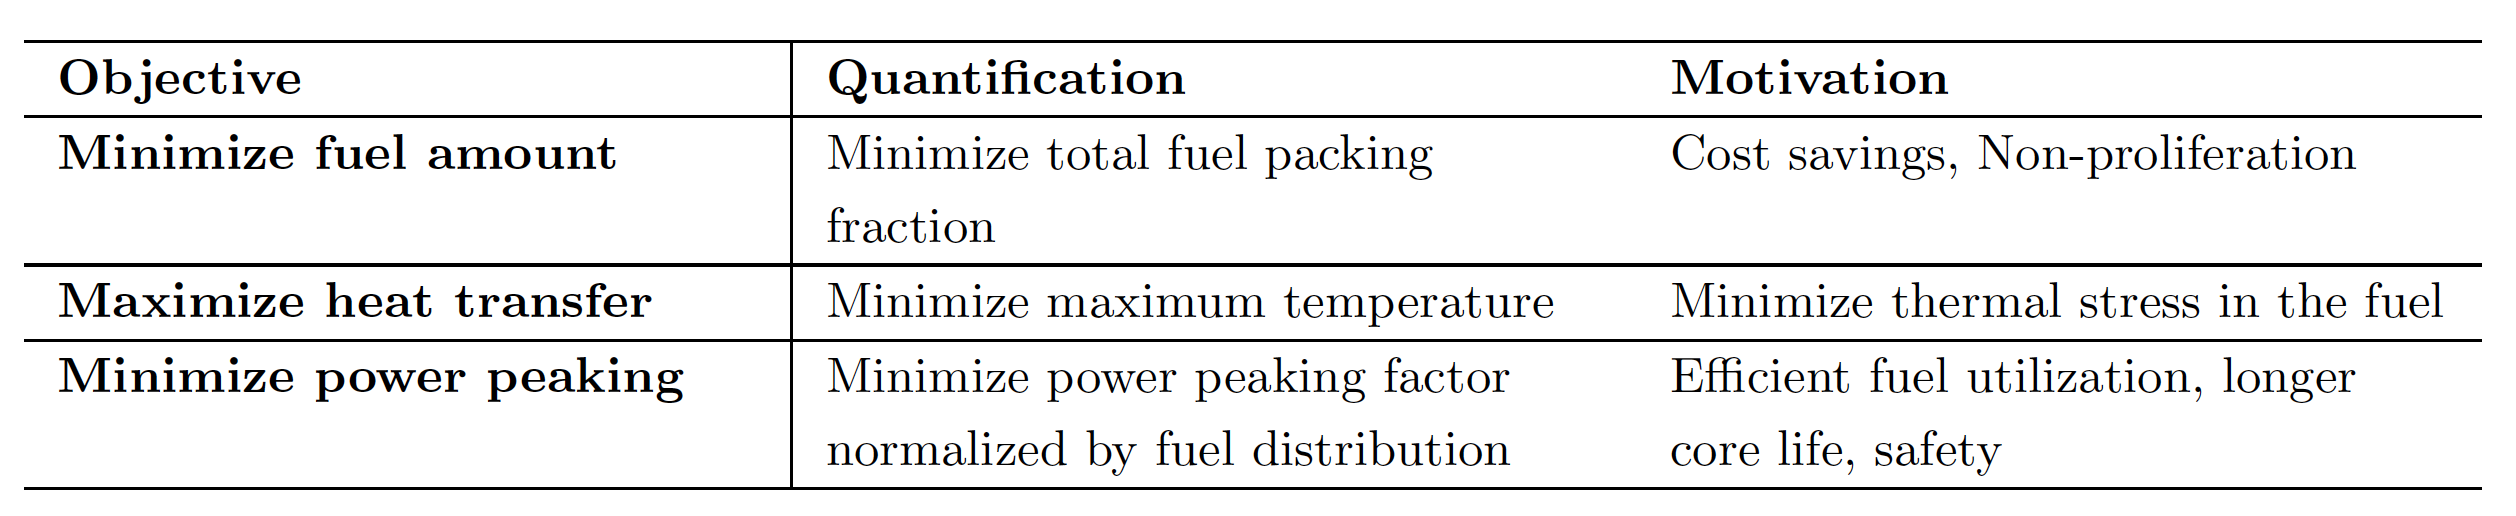
\includegraphics[width=0.9\linewidth]{figures/ahtr-opt-obj.png} 
            \caption{AHTR optimization problem objectives.}
        \end{figure}
    Maximum temperature ($T_{max}$), Normalized power peaking factor ($PPF_{fuel}$)
    \end{block}
\end{frame}

\begin{frame}
    \frametitle{AHTR One-Third Assembly Geometry}
    \begin{columns}
        \begin{column}{0.5\textwidth}
            Two sine distributions govern TRISO packing fraction distribution:
            \vspace{-0.2cm} 
            \begin{align}
            \rho_{TRISO}(\vec{x}, \vec{y}) &= \left(\textbf{a}\cdot sin(\textbf{b}\cdot 
            x + \textbf{c}) + 2\right) \nonumber \\
            & \cdot \left(\textbf{d}\cdot sin(\textbf{e}\cdot y + \textbf{f}) + 2\right) 
            \cdot NF \nonumber
            \end{align}
            \vspace{-0.7cm}
            \begin{figure}
                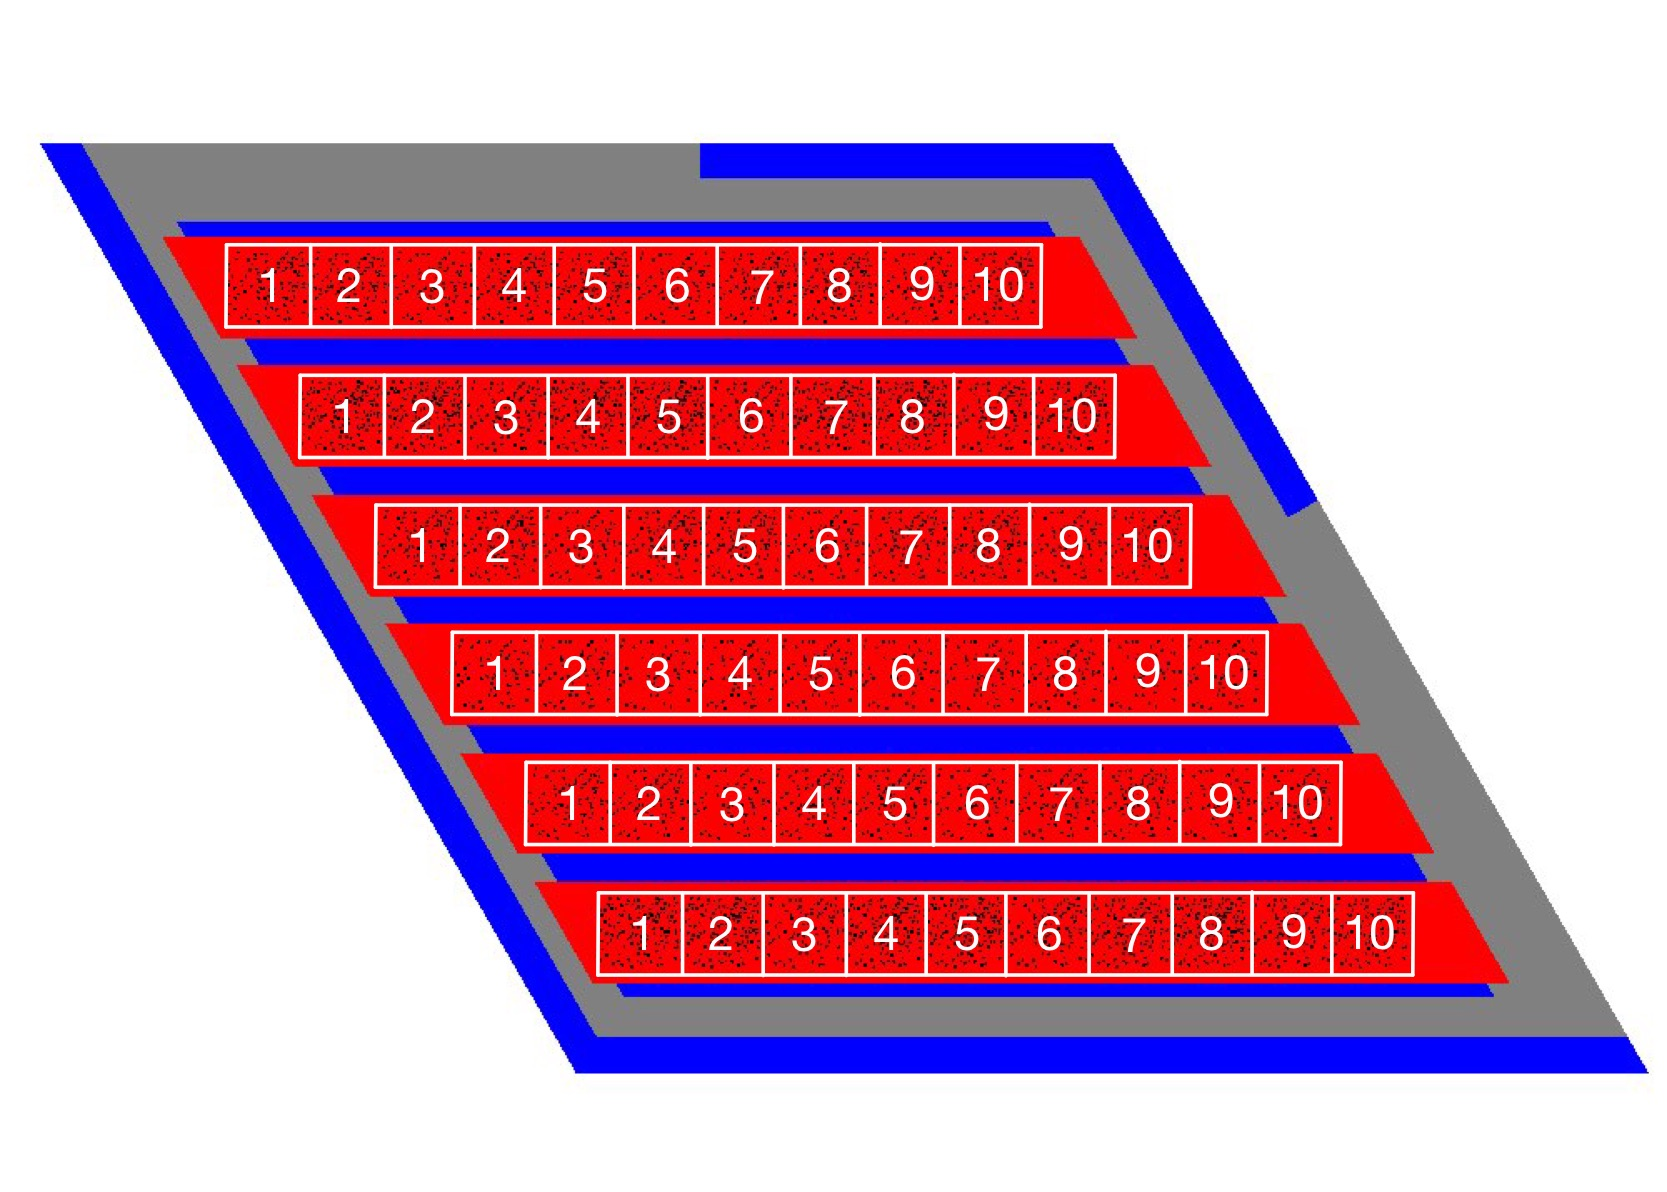
\includegraphics[width=\linewidth]{../docs/figures/ahtr_assembly.png} 
                \caption{AHTR one-third assembly with ten randomly packed fuel cells in 
                each graphite plank.}
            \end{figure}
        \end{column}
        \begin{column}{0.5\textwidth} 
            Five radius values (\textbf{$r_1, r_2, r_3, r_4, r_5$}) control coolant channel shape.
            \begin{figure}
                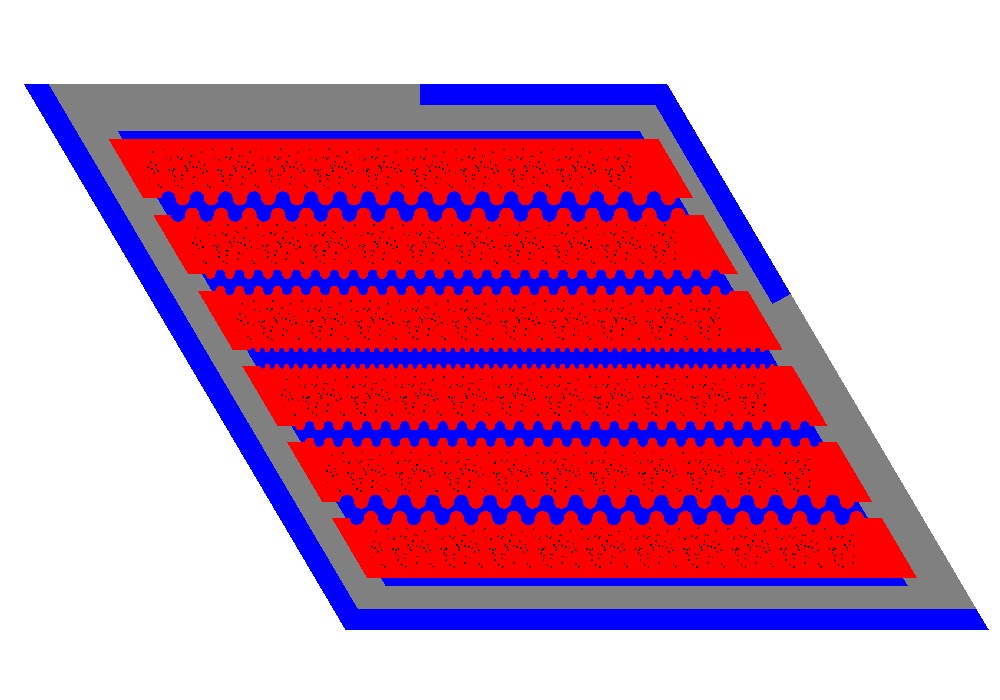
\includegraphics[width=\linewidth]{../docs/figures/coolant-channel-shape-assem.png} 
                \caption{AHTR one-third assembly with coolant channel shape variation, 
                $r_1, r_2, r_3, r_4, r_5$ = 0.3cm, 0.2cm, 0.1cm, 0.2cm, 0.3cm.}
            \end{figure}
        \end{column}
        \end{columns}
\end{frame}

% show a single obj workflow first and then full workflow.. step through it. 
\begin{frame}
    \frametitle{ROLLO AHTR Optimization Workflow}
    \begin{figure}
        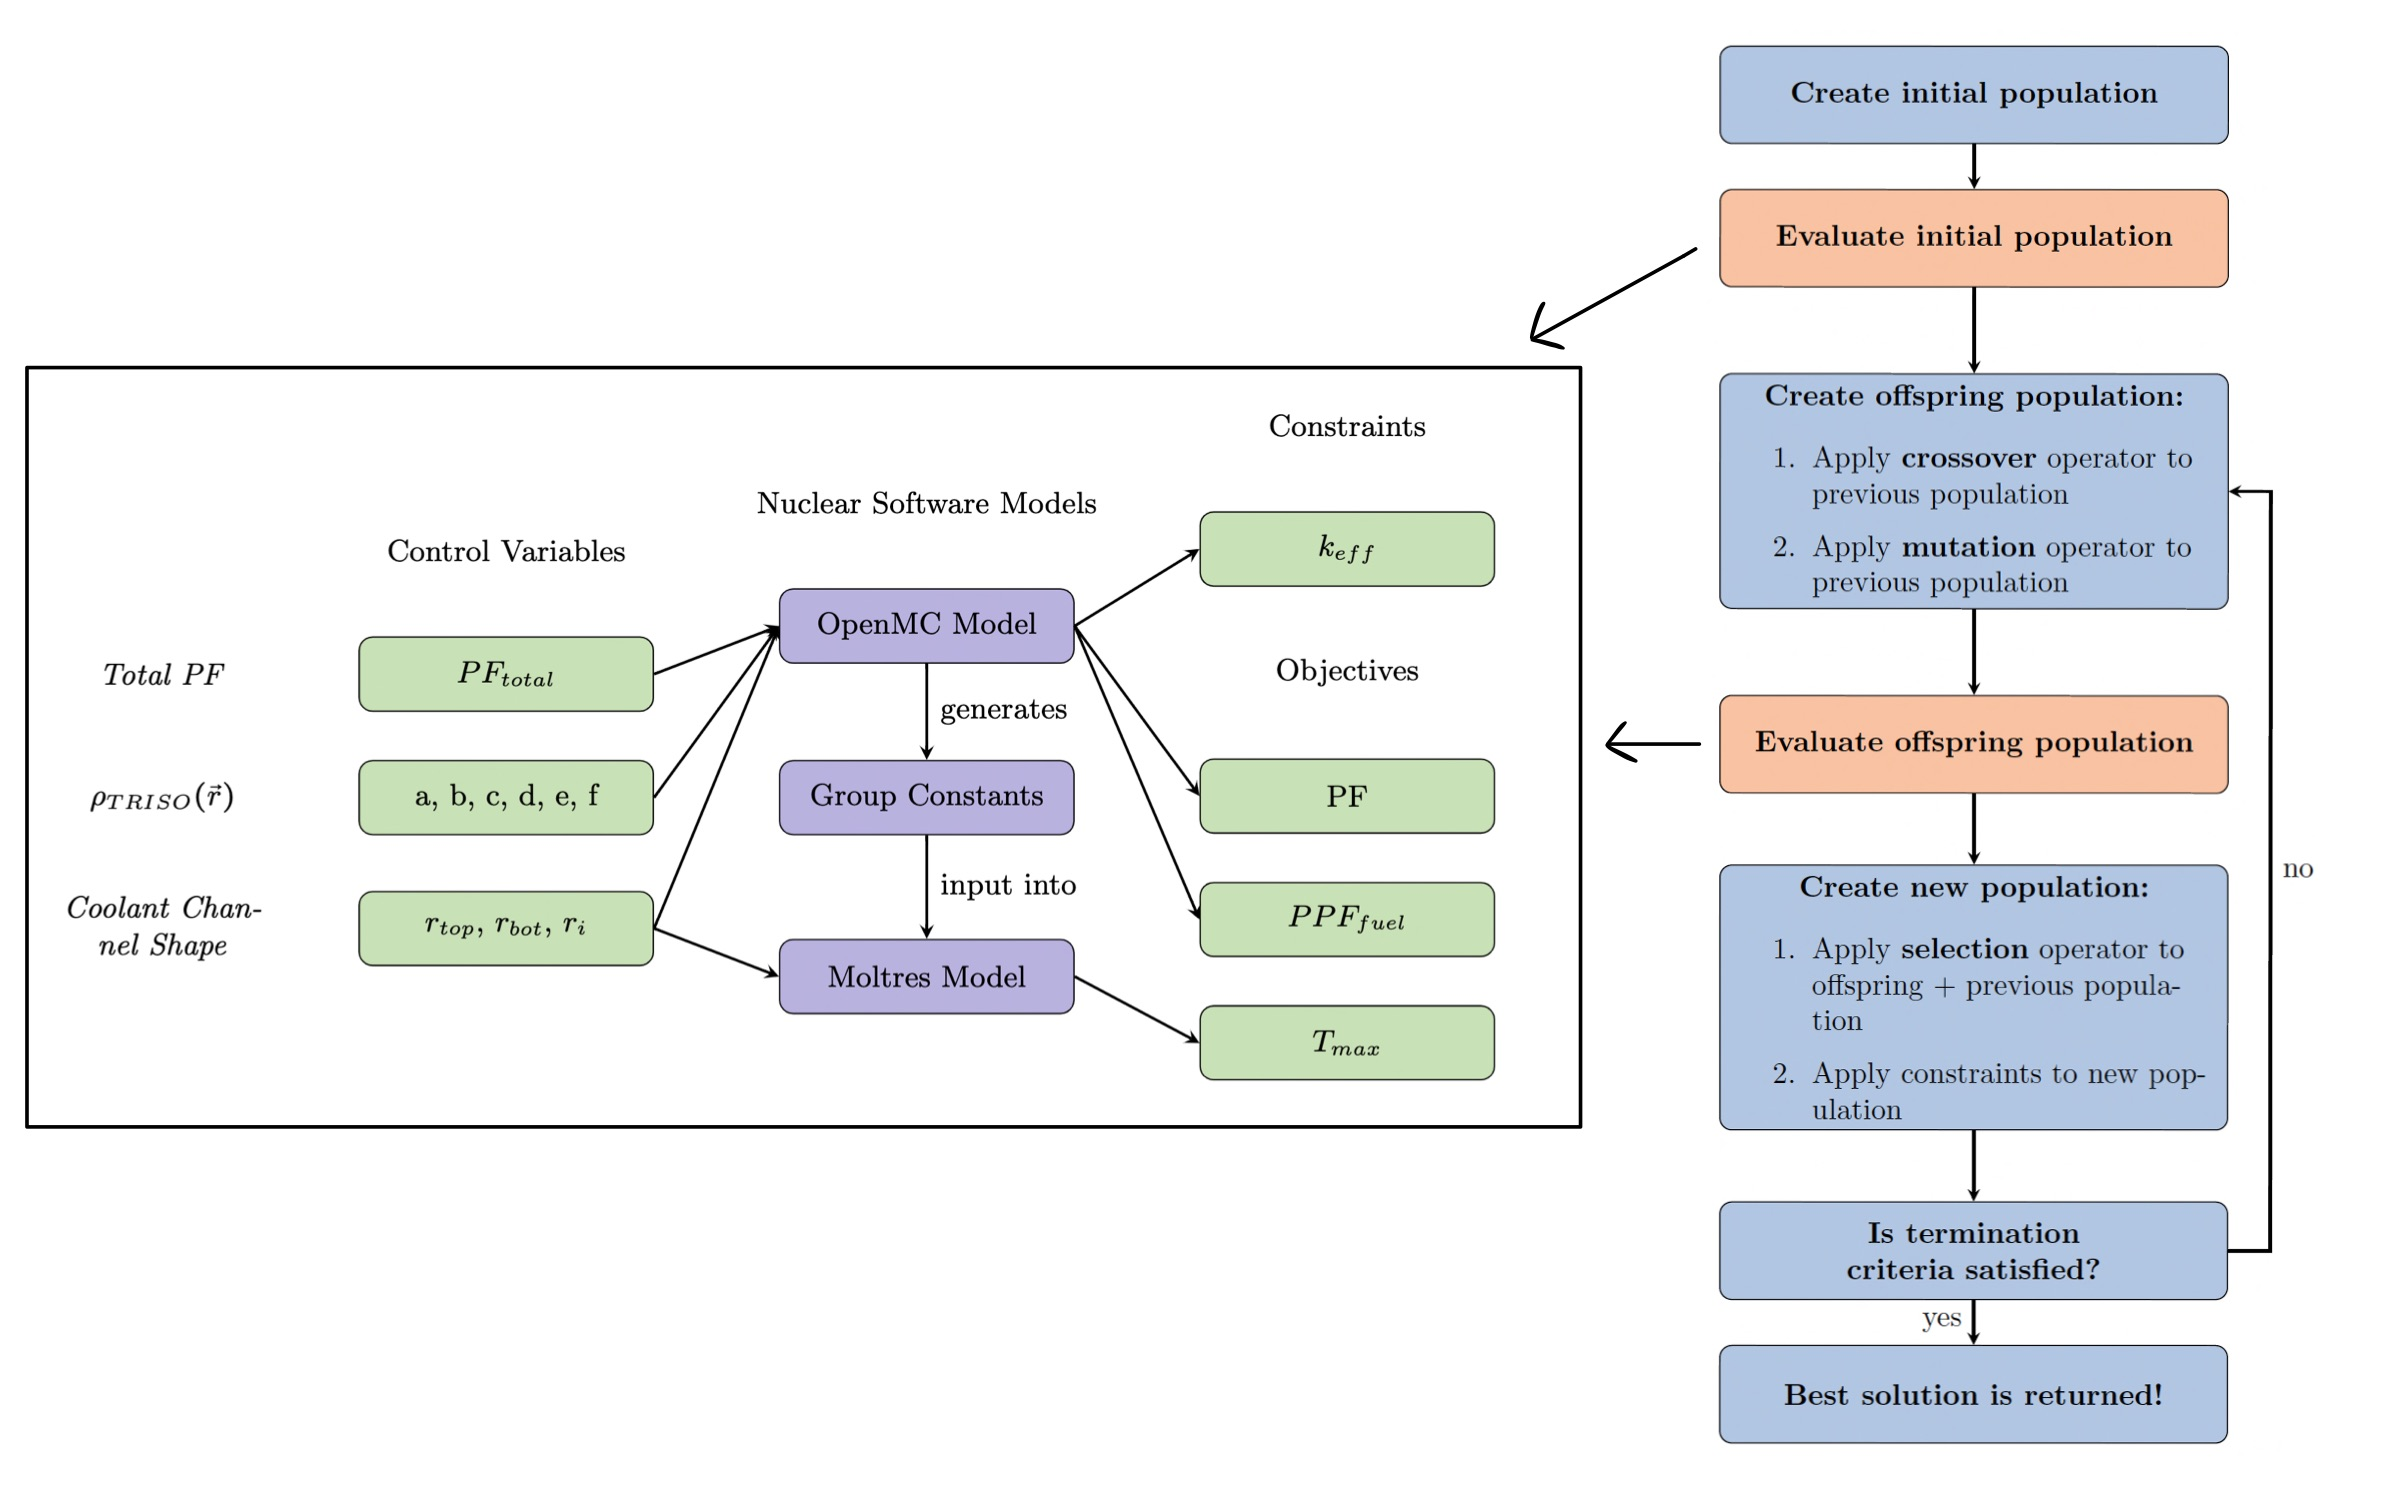
\includegraphics[width=0.9\linewidth]{figures/ahtr-modeling-workflow.png} 
        \caption{ROLLO AHTR Optimization Workflow.}
    \end{figure}
\end{frame}

% highlight which one i'm going to deep dive on 
\subsection{AHTR One-Third Assembly Optimization Results}
\begin{frame}
    \frametitle{AHTR One-Third Assembly Optimization Simulations}
    \only<1>{
        \begin{figure}
        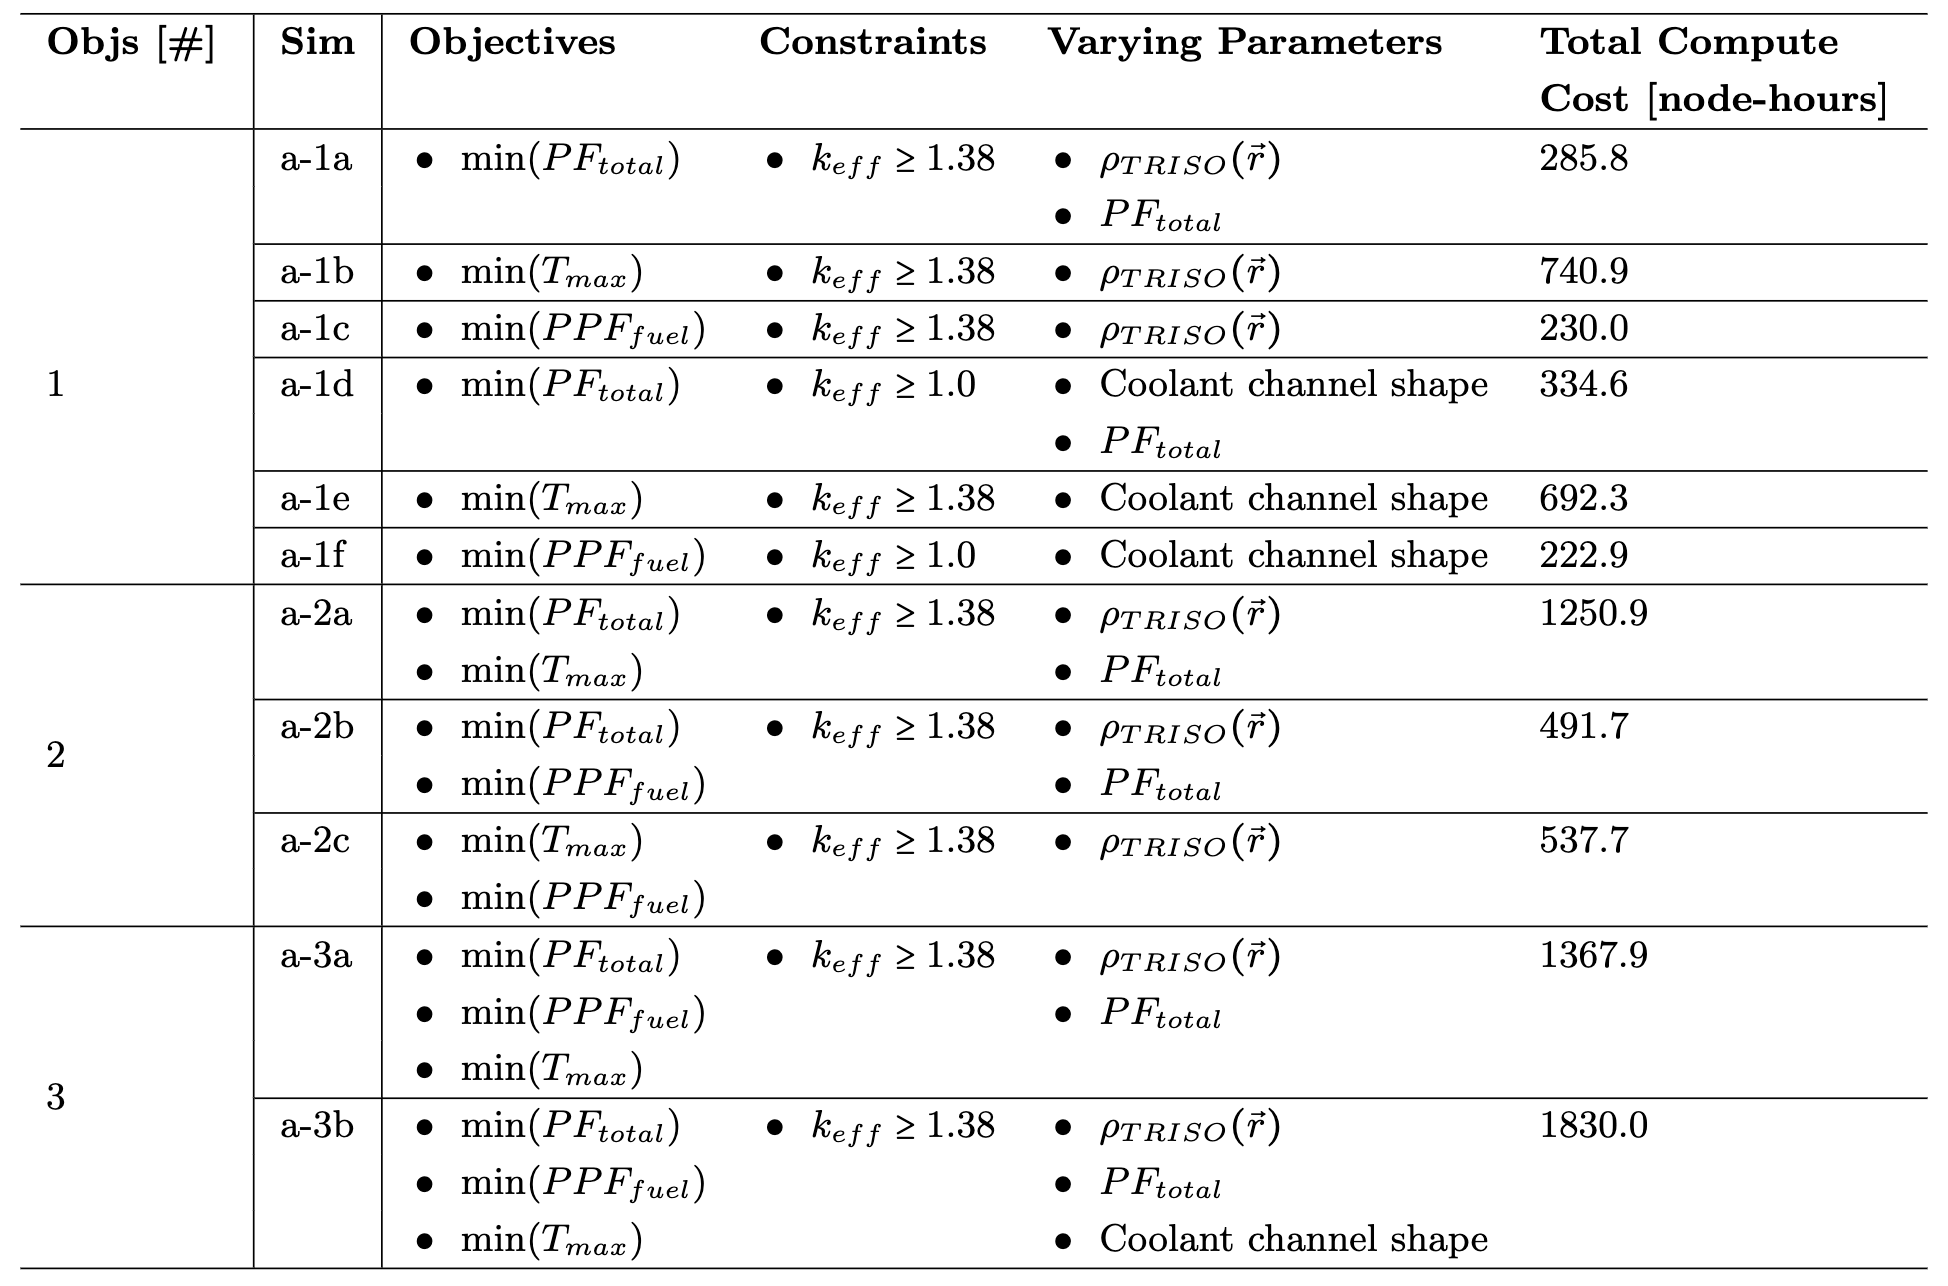
\includegraphics[width=0.85\linewidth]{figures/ahtr-assem-opt-table.png} 
        \caption{ROLLO simulations for optimizing the AHTR one-third assembly.}
        \end{figure}}
        \only<2>{
            \begin{figure}
            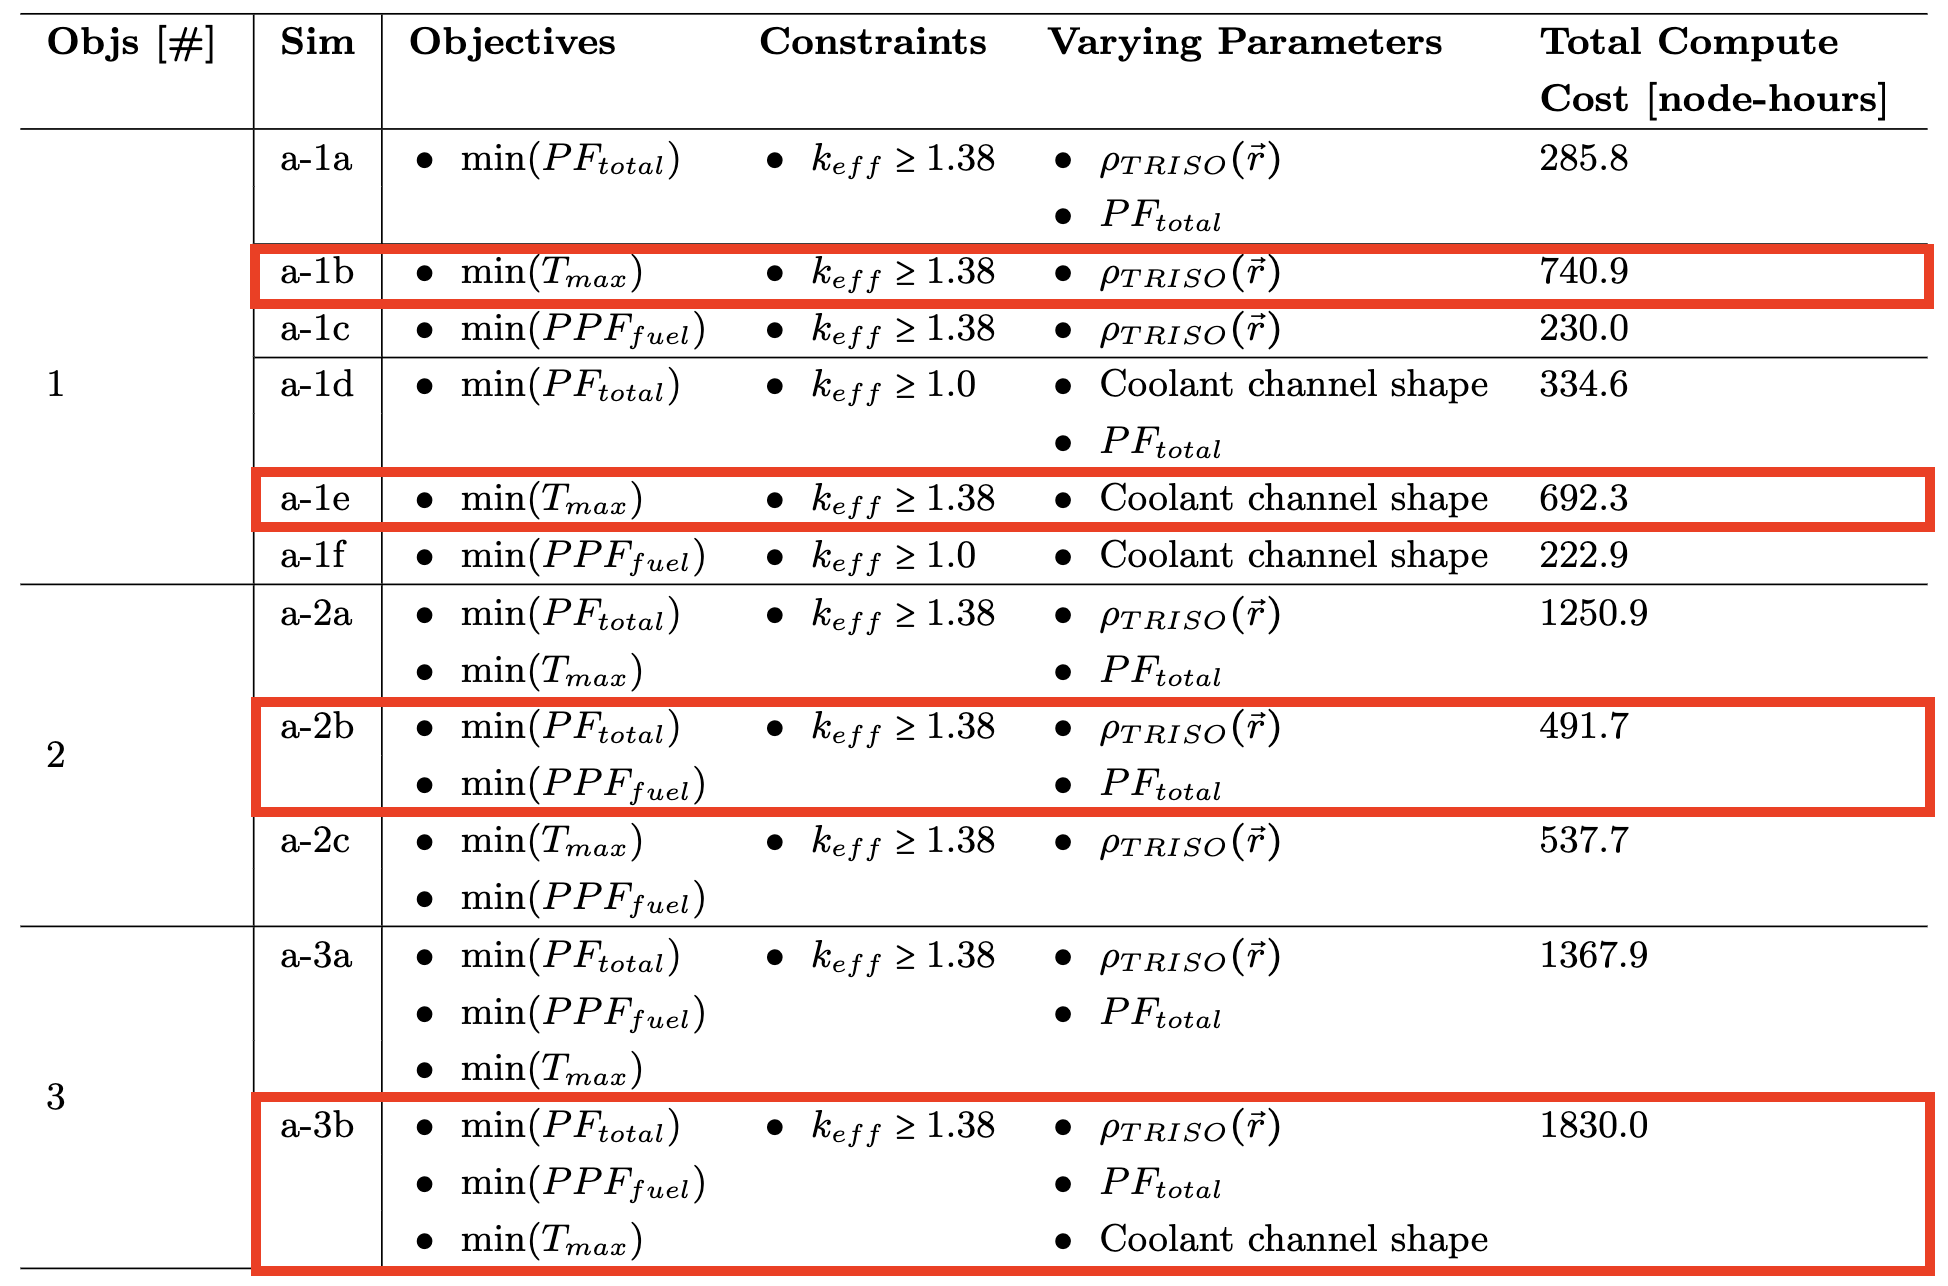
\includegraphics[width=0.8\linewidth]{figures/ahtr-assem-opt-table-annotated.png} 
            \caption{ROLLO simulations for optimizing the AHTR one-third assembly.}
            \end{figure}}
\end{frame}

\begin{frame}
    \frametitle{AHTR One-Third Assembly Simulation a-1b Results}
    I vary \textbf{a, b, c, d, e f} ($\rho_{TRISO}(\vec{x}, \vec{y}$))
    to minimize $T_{max}$. 

    \begin{figure}
        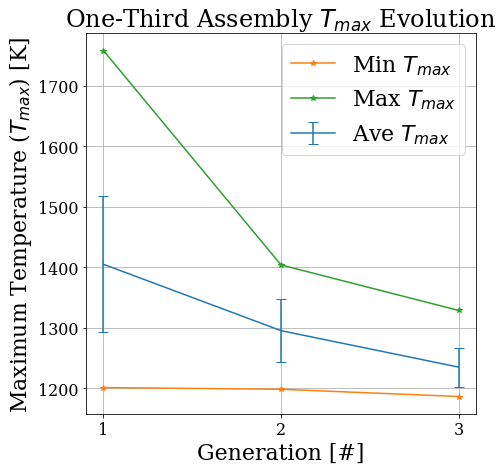
\includegraphics[width=0.39\linewidth]{figures/assem-obj-1-temp-evol-pres.png} 
        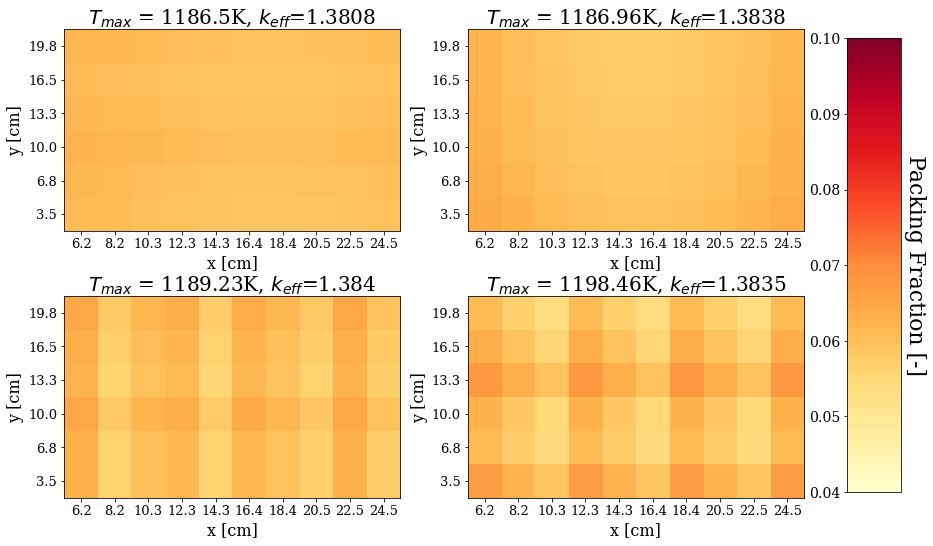
\includegraphics[width=0.59\linewidth]{../docs/figures/assem-obj-1-temp-final.png}
        \caption{Simulation a-1b $T_{max}$ evolution.}
    \end{figure}

    \begin{tcolorbox}[colback=illiniorange,colframe=illiniorange!50!black]
        \textbf{A flatter TRISO distribution minimizes $T_{max}$.}
    \end{tcolorbox}
\end{frame}

\begin{frame}
    \frametitle{AHTR One-Third Assembly Simulation a-1e Results}
    I vary $r_1, r_2, r_3, r_4, r_5$ (coolant channel shape)
    to minimize $T_{max}$. 
    \begin{figure}
        \centering
        \begin{subfigure}{0.3\textwidth}
            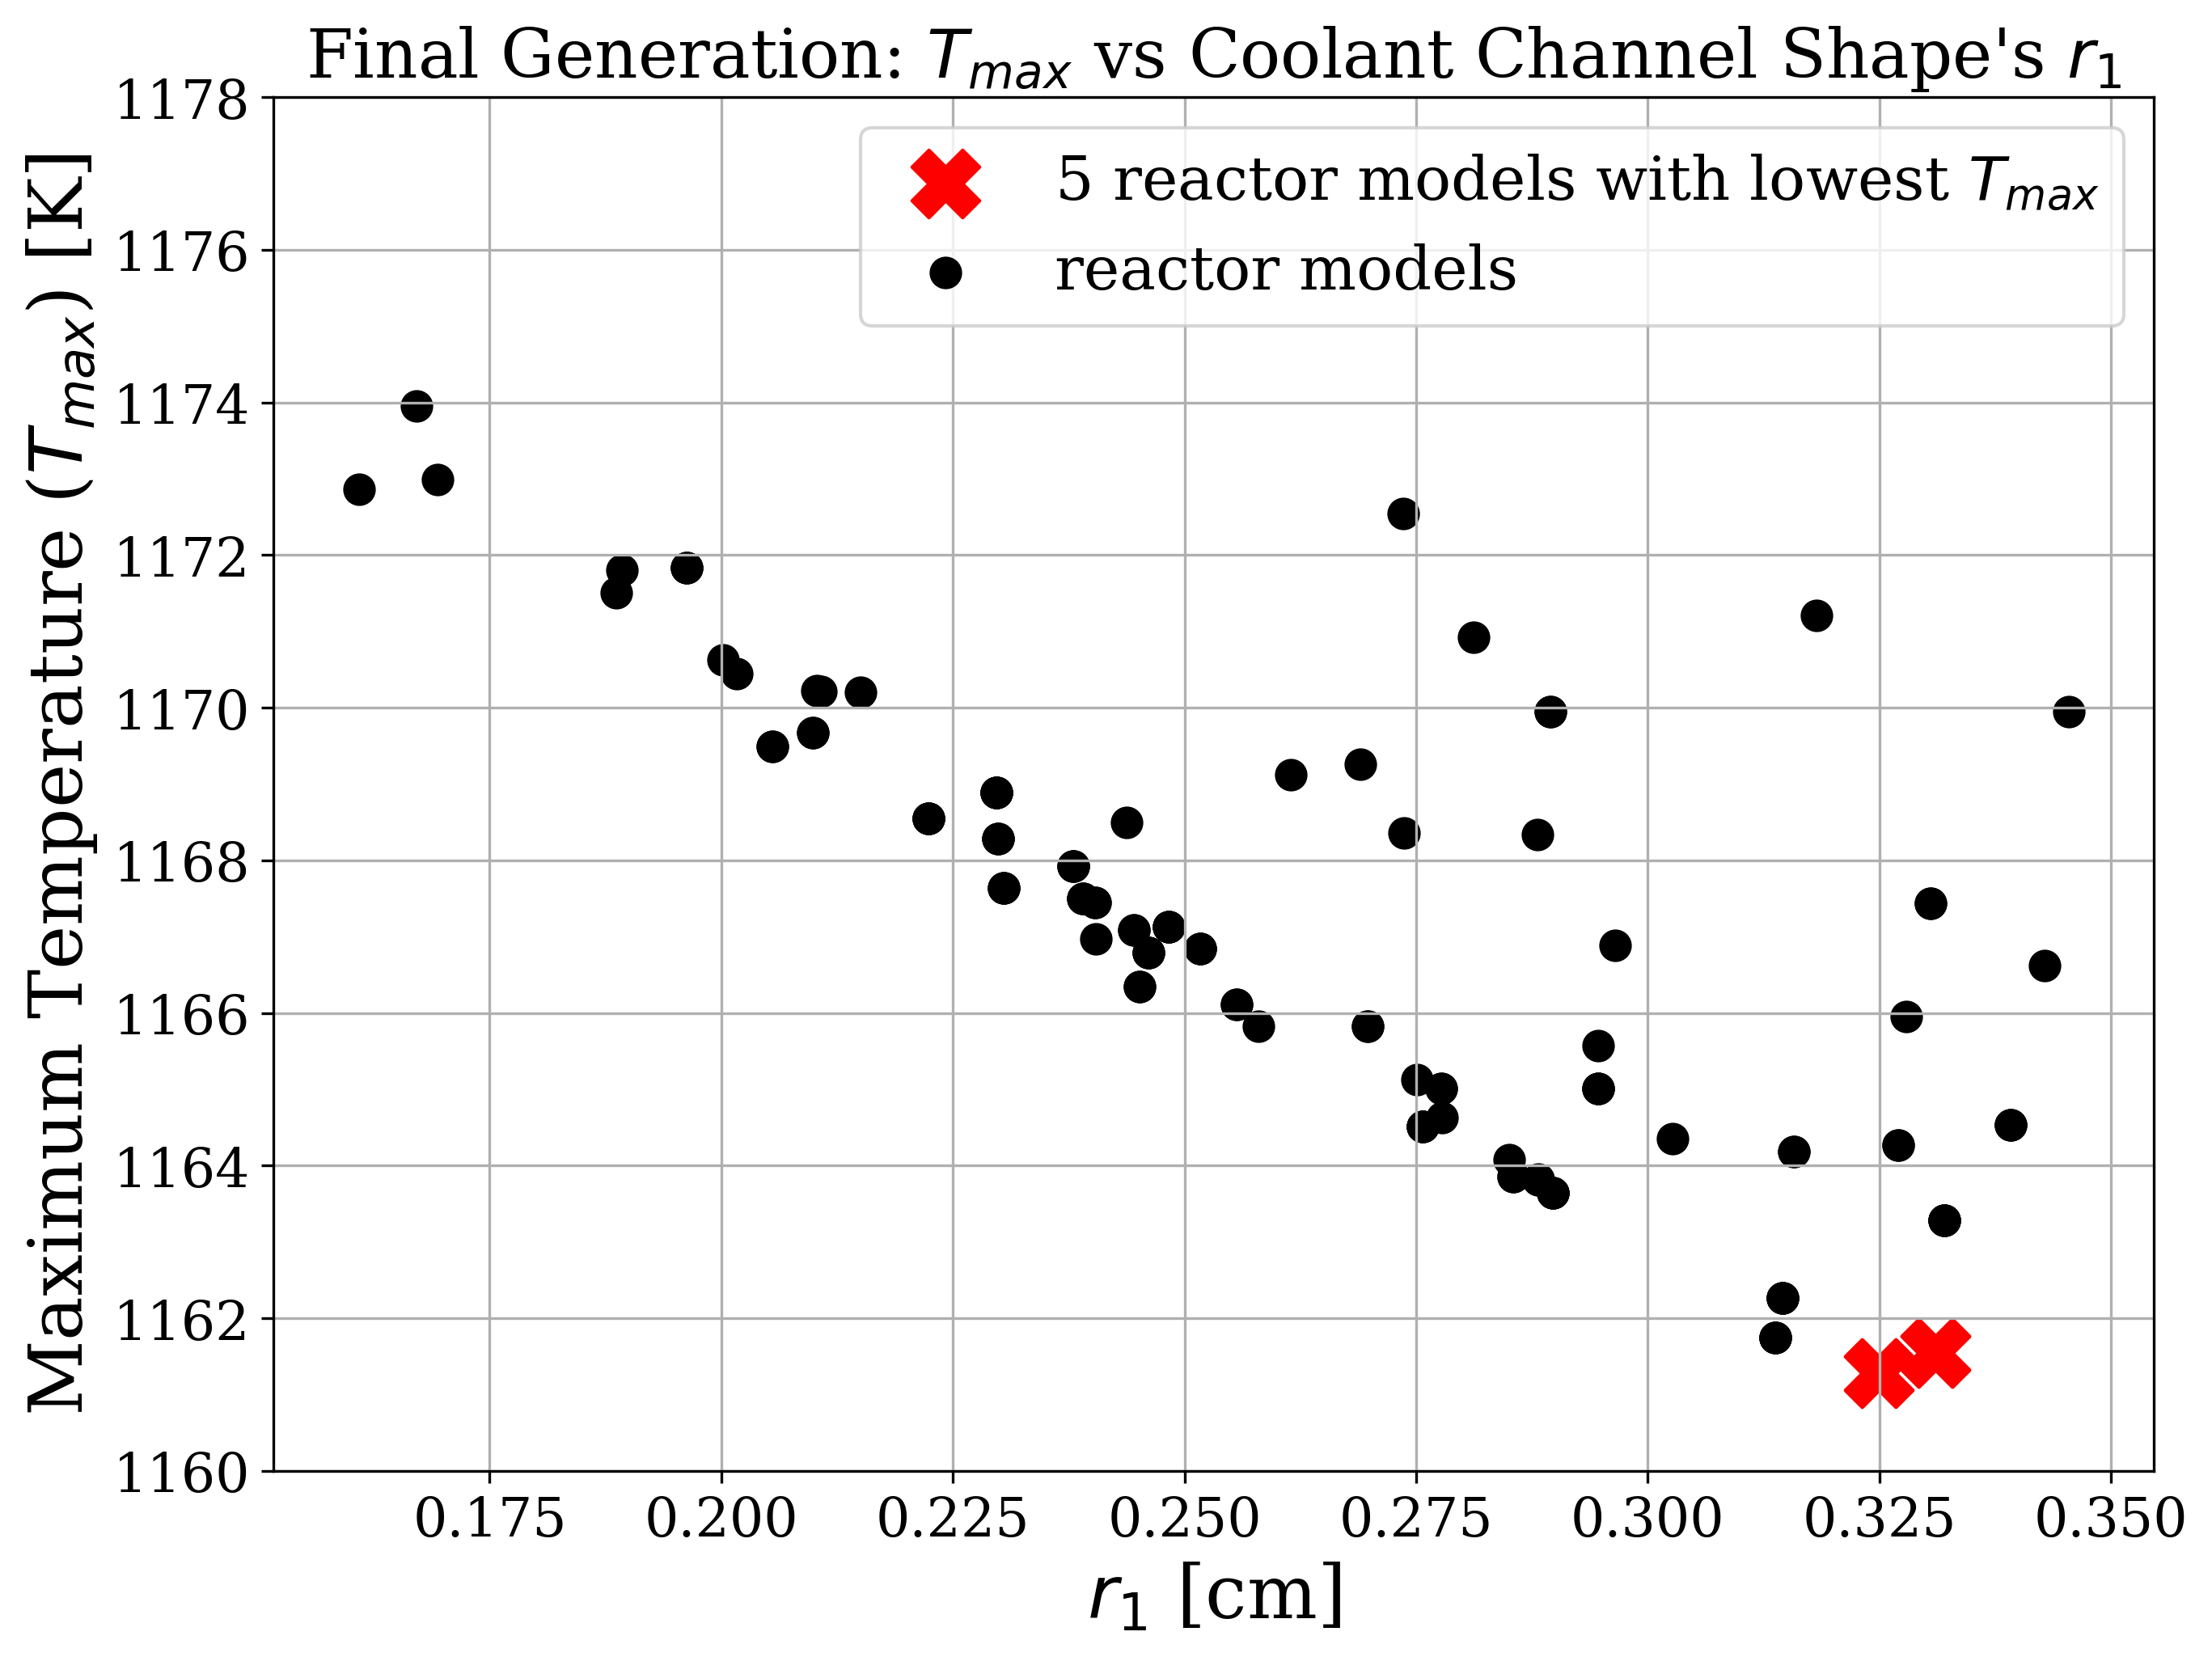
\includegraphics[width=\linewidth]{../docs/figures/a-1e-r1.png}
            \caption{Plot of $T_{max}$ against $r_1$.}
            \label{fig:a-1e-r1} 
        \end{subfigure}
        \begin{subfigure}{0.3\textwidth}
            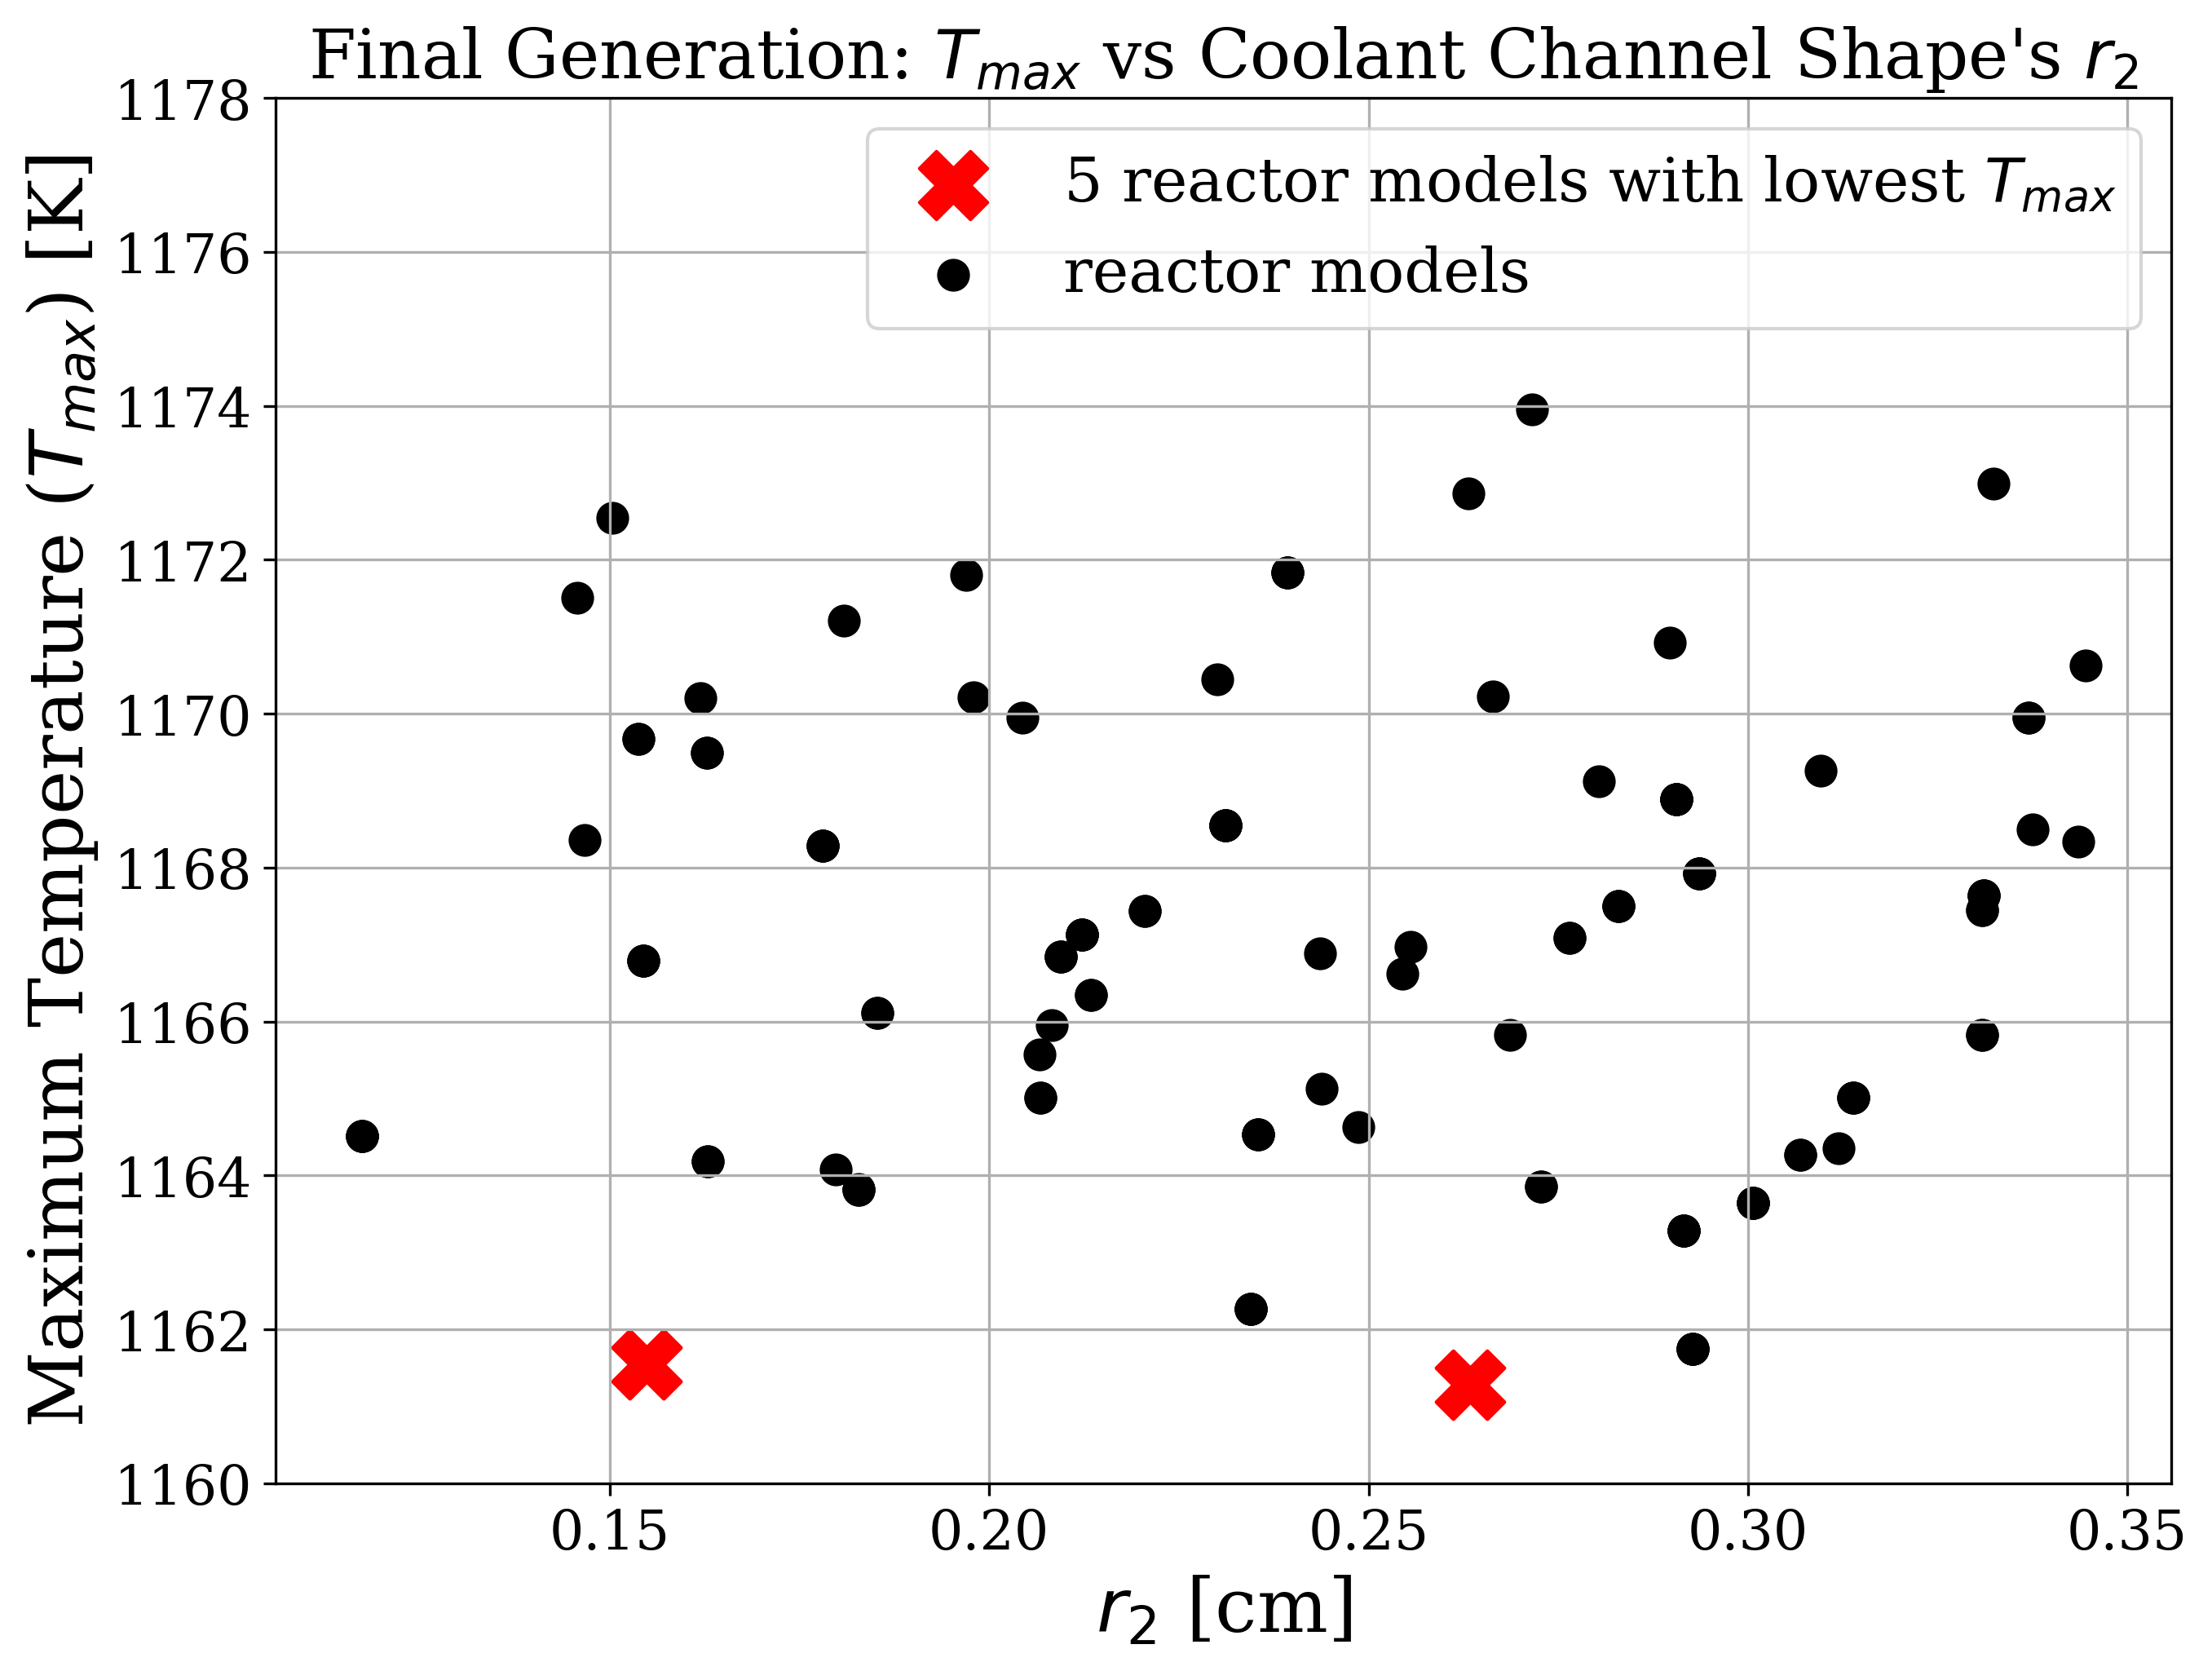
\includegraphics[width=\linewidth]{../docs/figures/a-1e-r2.png}
            \caption{Plot of $T_{max}$ against $r_2$.}
            \label{fig:a-1e-r2} 
        \end{subfigure}
        \begin{subfigure}{0.3\textwidth}
            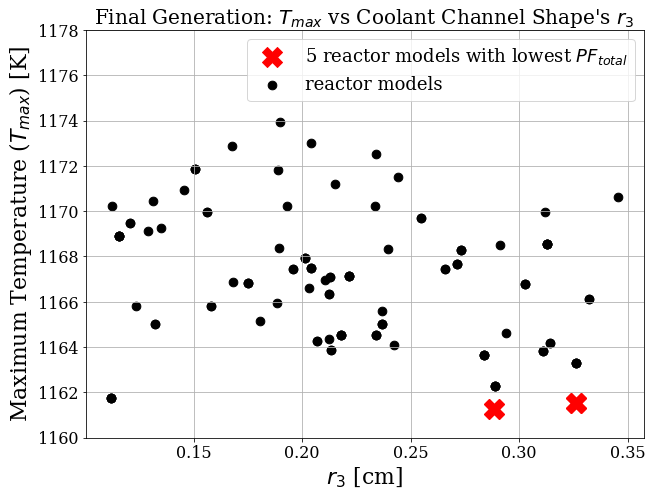
\includegraphics[width=\linewidth]{../docs/figures/a-1e-r3.png}
            \caption{Plot of $T_{max}$ against $r_3$.}
            \label{fig:a-1e-r3} 
        \end{subfigure}
        \begin{subfigure}{0.3\textwidth}
            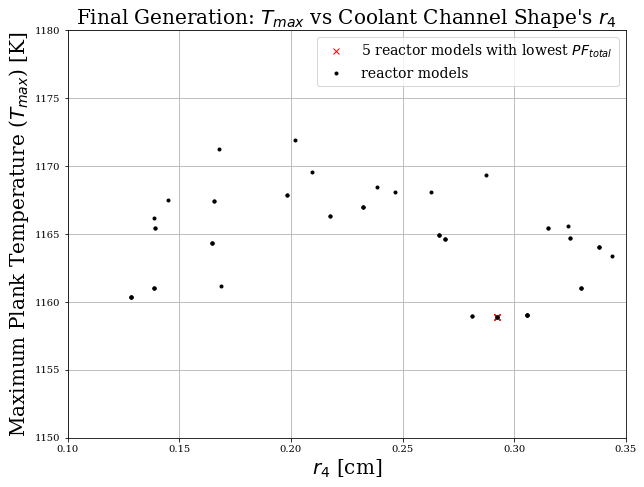
\includegraphics[width=\linewidth]{../docs/figures/a-1e-r4.png}
            \caption{Plot of $T_{max}$ against $r_4$.}
            \label{fig:a-1e-r4} 
        \end{subfigure}
        \begin{subfigure}{0.3\textwidth}
            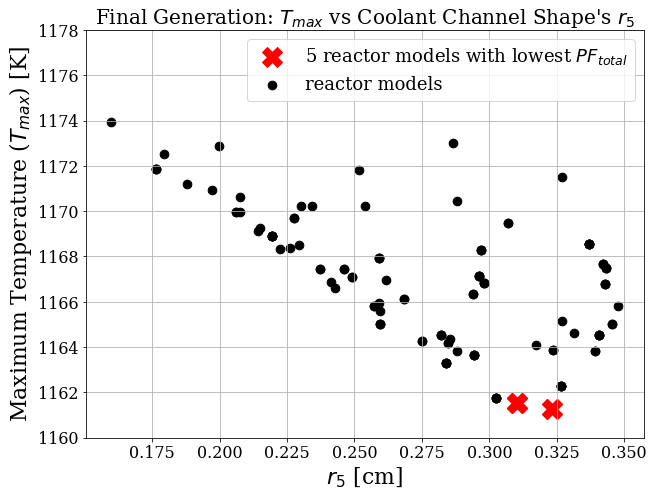
\includegraphics[width=\linewidth]{../docs/figures/a-1e-r5.png}
            \caption{Plot of $T_{max}$ against $r_5$.}
            \label{fig:a-1e-r5} 
        \end{subfigure}
        \caption{Simulation a-1e.}
    \end{figure}
\end{frame}

\begin{frame}
    \frametitle{AHTR One-Third Assembly Simulation a-1e Results}
    \begin{figure}
        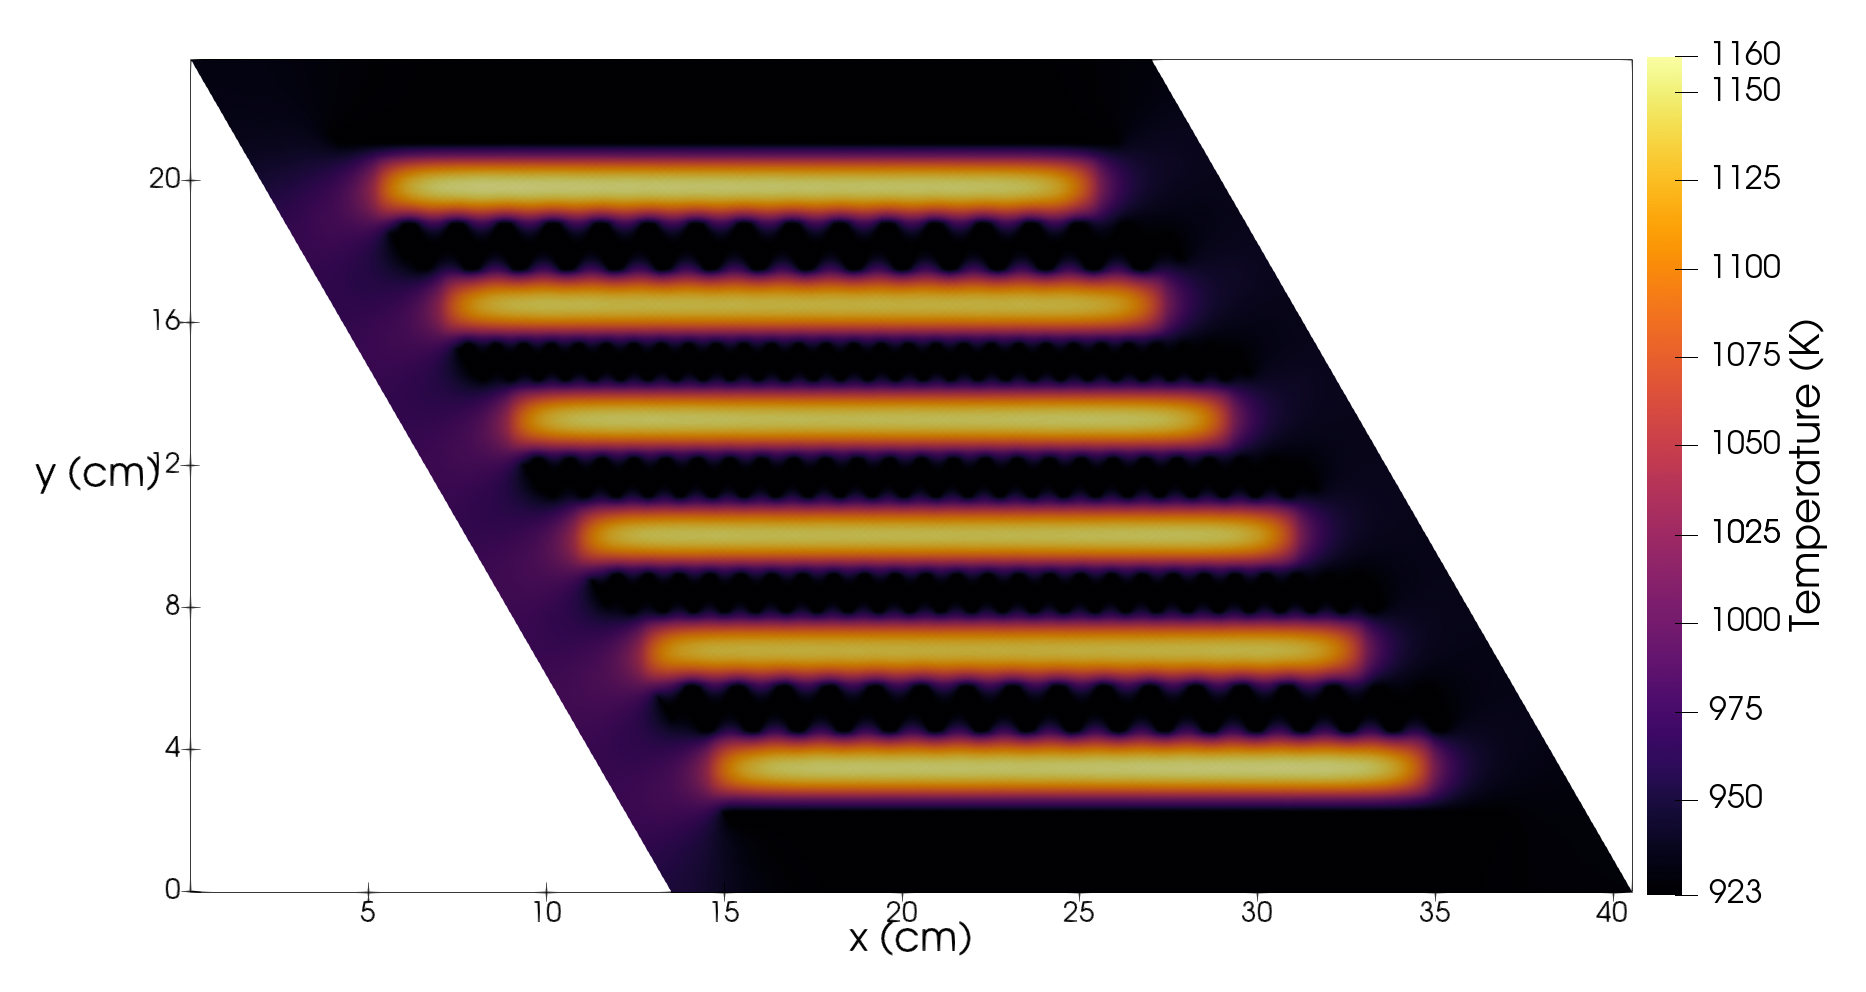
\includegraphics[width=0.55\linewidth]{../docs/figures/a-1e-temp-distribution-2d.png} 
        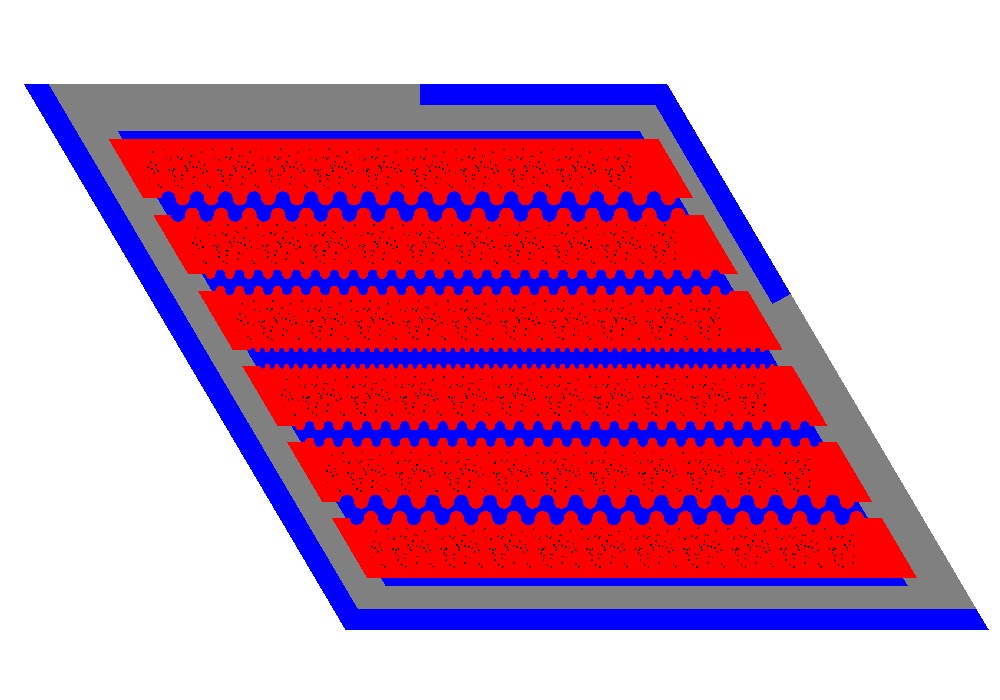
\includegraphics[width=0.4\linewidth]{../docs/figures/coolant-channel-shape-assem.png} 
        \caption{Temperature Distribution in simulation a-1e's most-minimized $T_{max}$ reactor 
        model.}
    \end{figure}
    \begin{tcolorbox}[colback=illiniorange,colframe=illiniorange!50!black]
    \textbf{FLiBe channels located closest to temperature peaks shows a \\ negative 
    correlation with $T_{max}$.}
    \end{tcolorbox}
\end{frame}

\begin{frame}
    \frametitle{Single-Objective Optimization Major Takeaways}
    \textbf{Minimize $PF_{total}$ Objective} 
    \begin{itemize}
        \item Driven by maximizing total fission reaction rate
        \item Influences oscillations in TRISO's spatial distribution
        \item No correlation with coolant channel shape  
    \end{itemize}

    \textbf{Minimize $T_{max}$ Objective}
    \begin{itemize}
        \item A flatter TRISO distribution minimizes $T_{max}$
        \item FLiBe channels located closest to temperature peaks shows a negative 
        correlation with $T_{max}$
    \end{itemize}

    \textbf{Minimize $PPF_{fuel}$ Objective} 
    \begin{itemize}
        \item Driven by flattening thermal flux distribution
        \item Influences oscillations in TRISO's spatial distribution
        \item No correlation with coolant channel shape  
    \end{itemize}
\end{frame}


\begin{frame}
    \frametitle{AHTR One-Third Assembly Simulation a-2b Results}
    I vary $PF_{total}$ and \textbf{a, b, c, d, e f} ($\rho_{TRISO}(\vec{x}, \vec{y}$))
    to minimize $PF_{total}$ and $PPF_{fuel}$. 
    \begin{figure}
        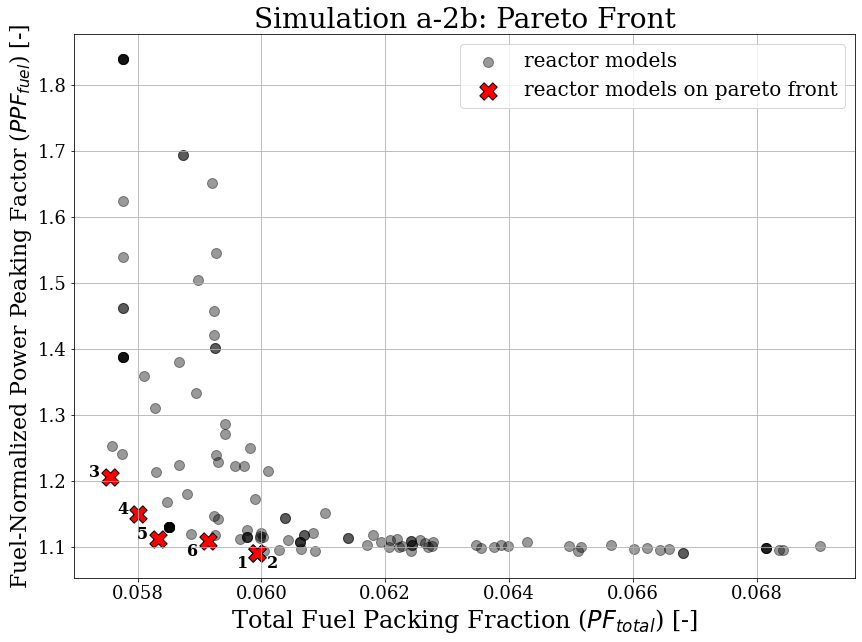
\includegraphics[width=0.65\linewidth]{../docs/figures/assem-obj-2-pfppf-pareto.png} 
        \caption{Simulation a-2b Pareto Front.}
    \end{figure}
\end{frame}

\begin{frame}
    \frametitle{AHTR One-Third Assembly Simulation a-2b Results}
    \only<1>{
    \begin{figure}
        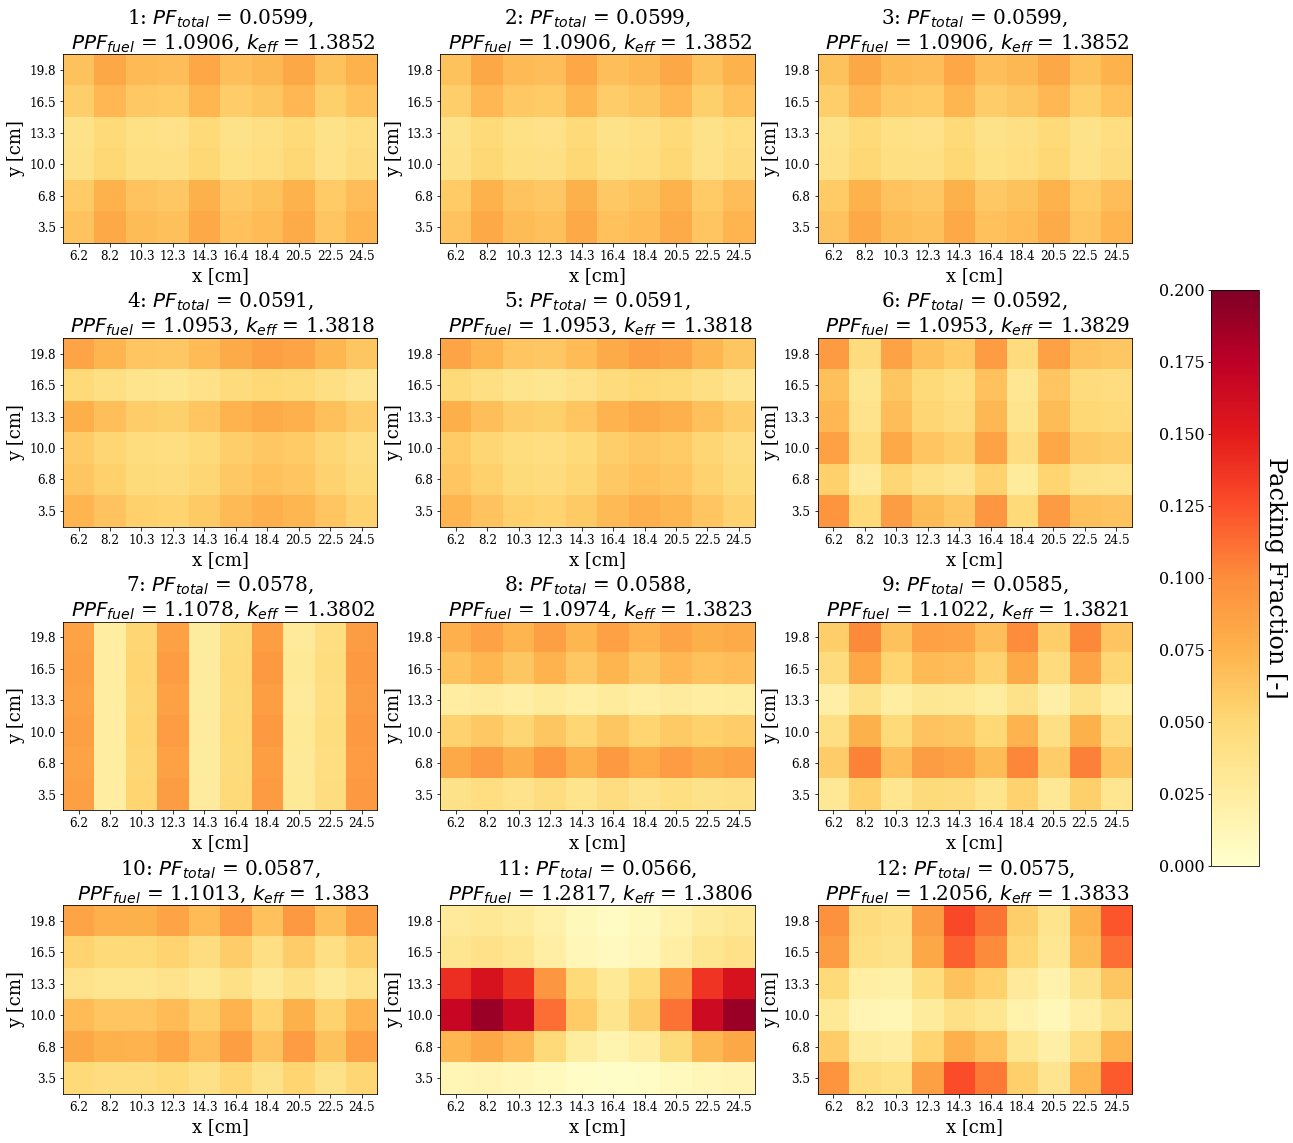
\includegraphics[width=0.8\linewidth]{../docs/figures/assem-obj-2-pfppf-pareto-distr.png}
        \caption{Simulation a-2b Pareto Front's TRISO Distributions.}
    \end{figure}}
    \only<2>{
    \begin{figure}
        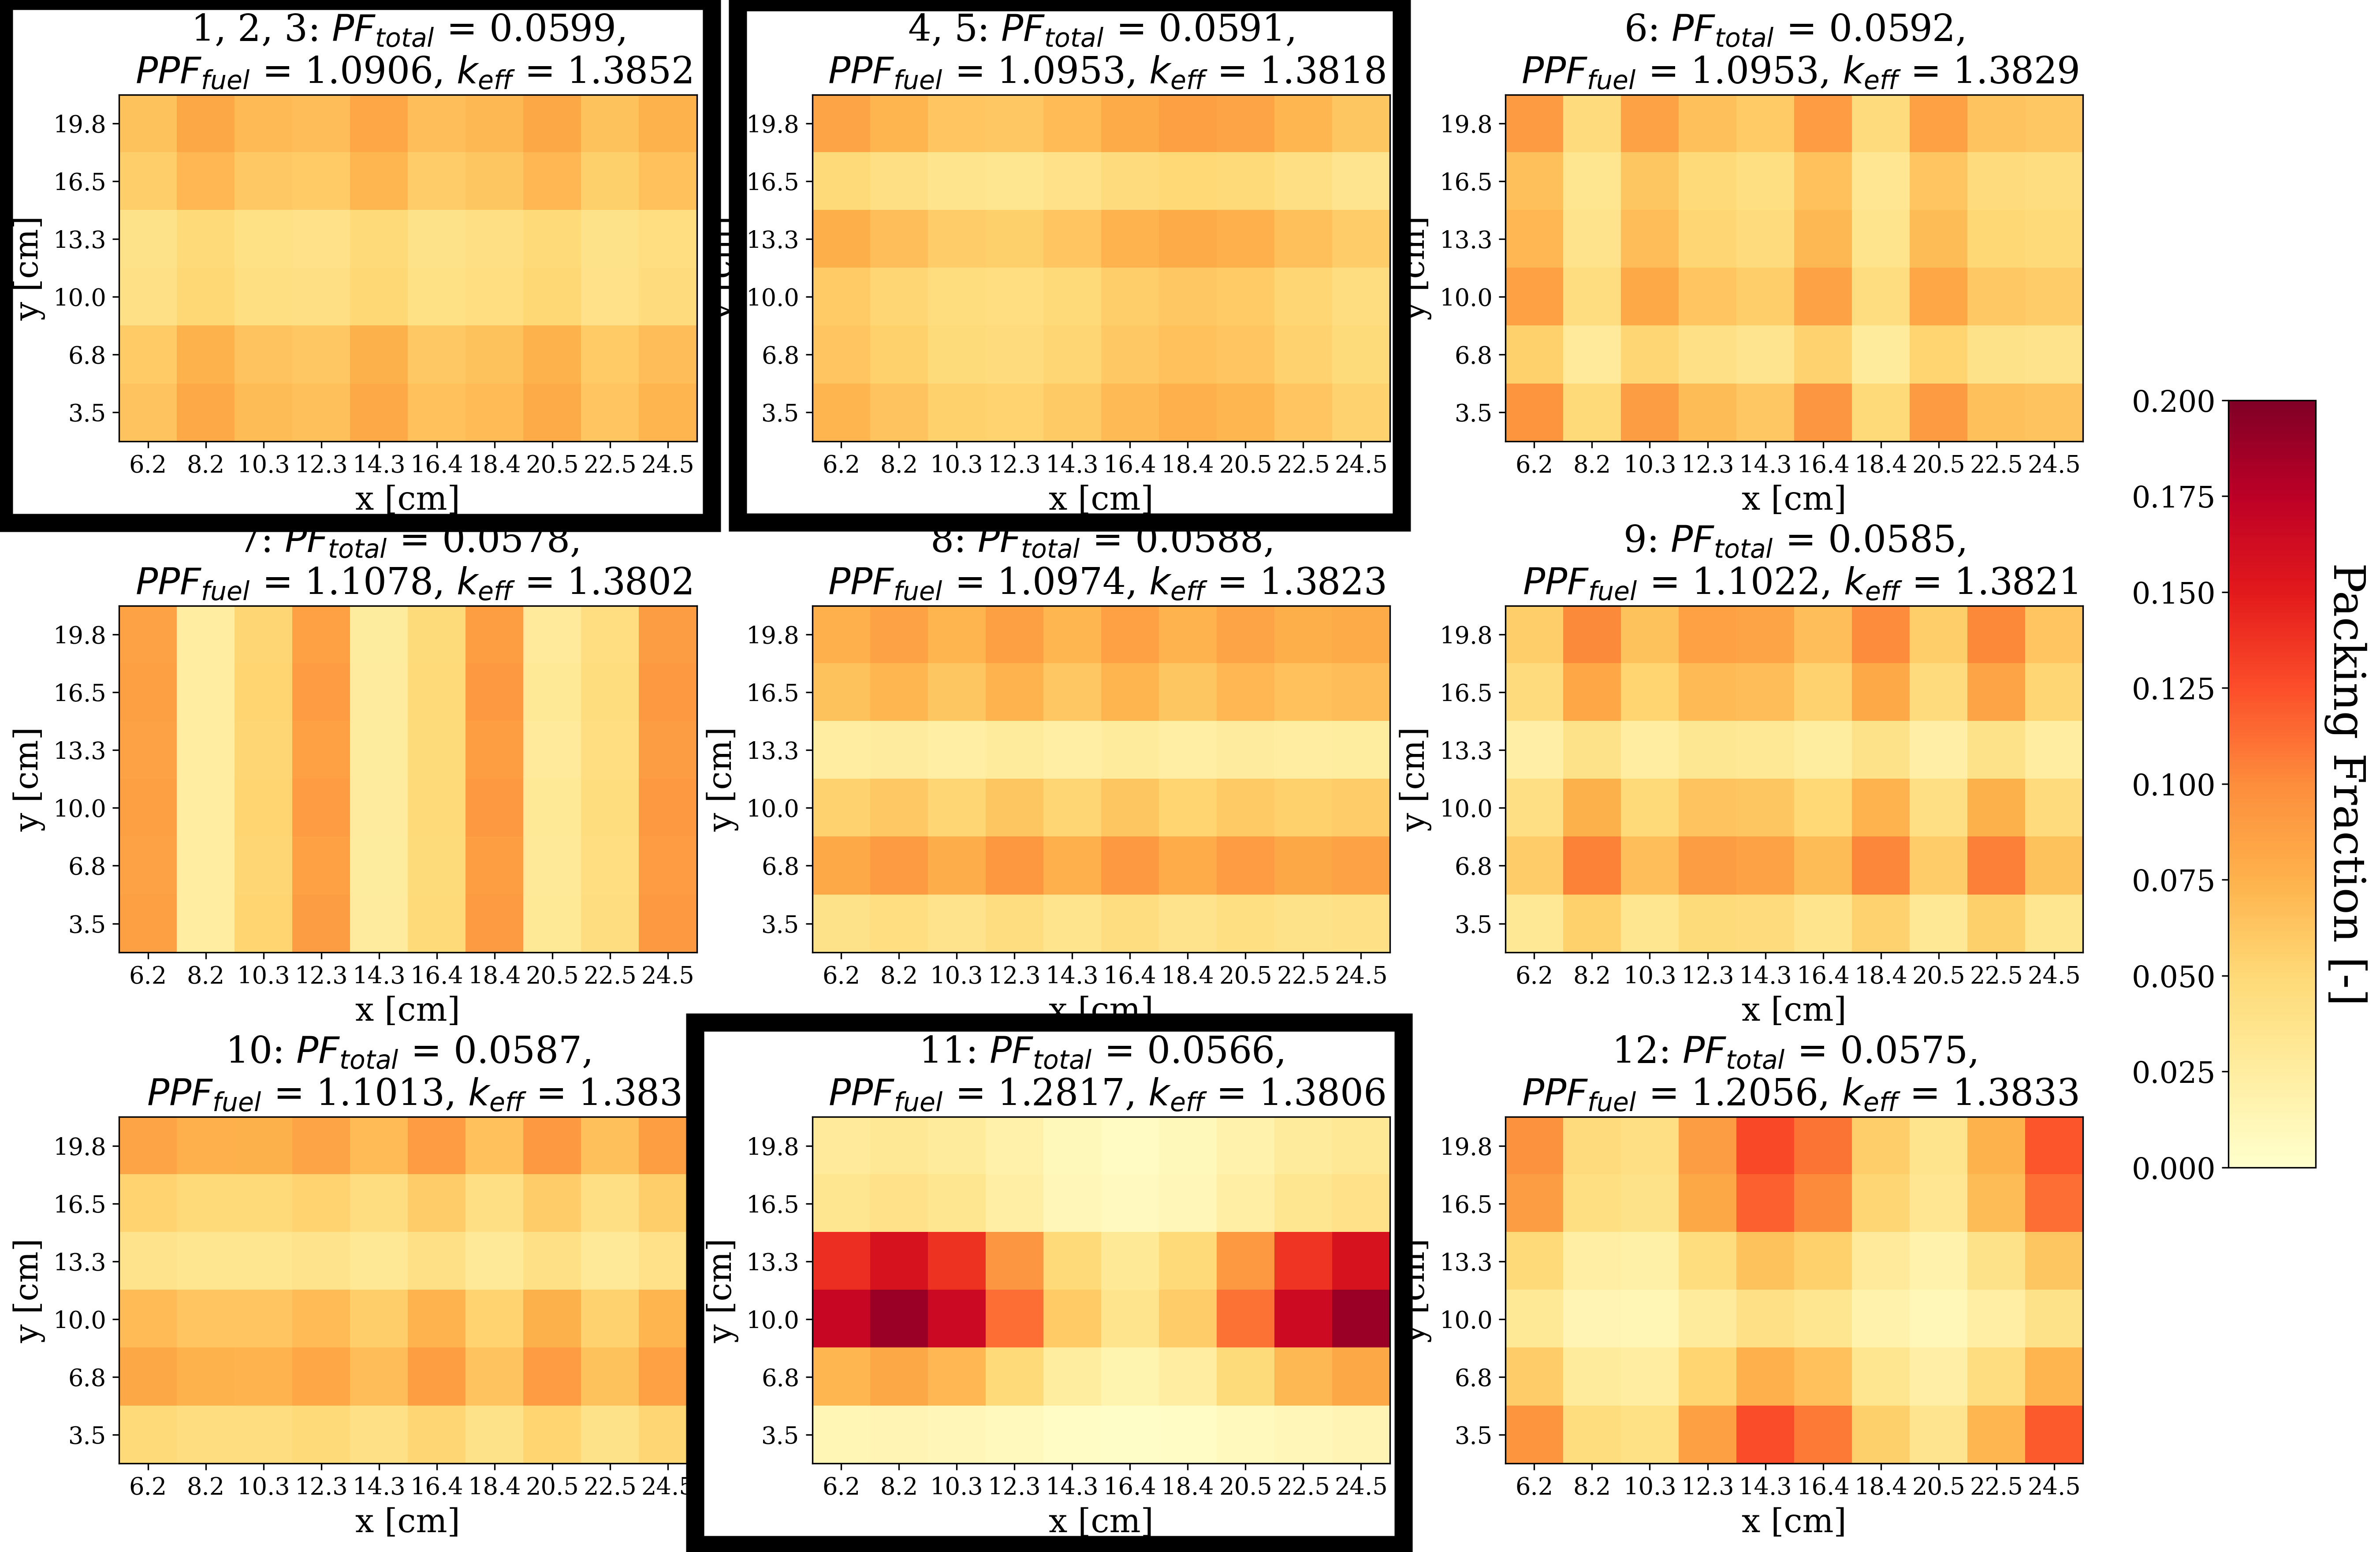
\includegraphics[width=0.8\linewidth]{figures/assem-obj-2-pfppf-pareto-distr-annotated.png}
        \caption{Simulation a-2b Pareto Front's TRISO Distributions.}
    \end{figure}}
\end{frame}

\begin{frame}
    \frametitle{AHTR One-Third Assembly Simulation a-2b Results}
    Minimize $PF_{total}$ objective is driven by \textbf{maximizing 
    total fission reaction rate}. \\
    Minimize $PPF_{fuel}$ objective is driven by \textbf{flattening 
    thermal flux distribution}. 

    \begin{figure}
        \centering
        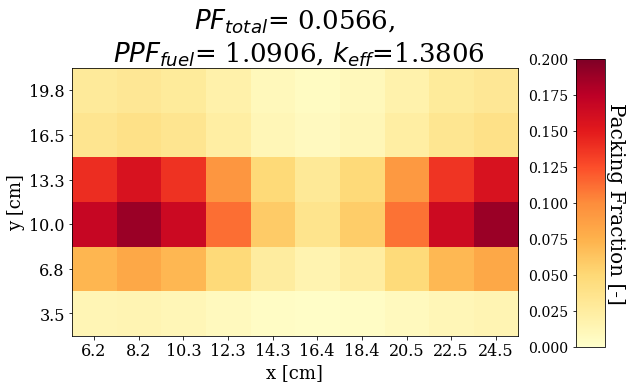
\includegraphics[width=0.37\linewidth]{../docs/figures/a-2b-pf-most-minimized.png} 
        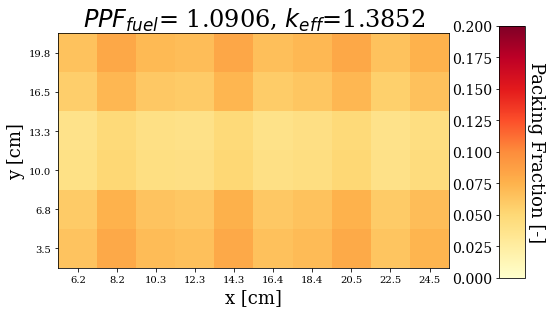
\includegraphics[width=0.37\linewidth]{../docs/figures/a-2b-ppf-most-minimized.png} 
        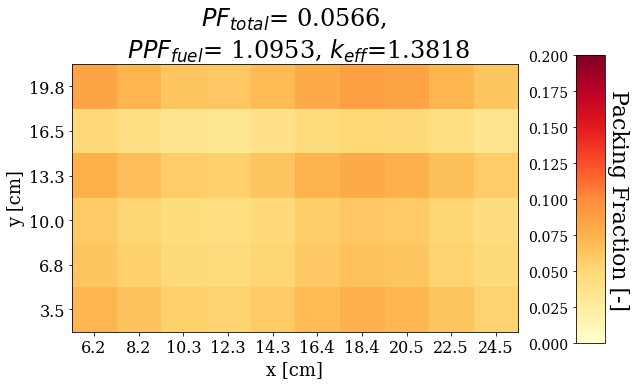
\includegraphics[width=0.37\linewidth]{../docs/figures/a-2b-both-most-minimized.png}
        \caption{Simulation a-2b Pareto Front's TRISO Distributions.}
    \end{figure}
    \vspace{-0.2cm}
    Minimize $PF_{total}$ and Minimize $PPF_{fuel}$ objectives \textbf{influence TRISO distribution}. 
\end{frame}

\begin{frame}
    \frametitle{AHTR One-Third Assembly Simulation a-3b Results}
    \begin{columns}
    \begin{column}{0.7\textwidth}
    \begin{figure}
        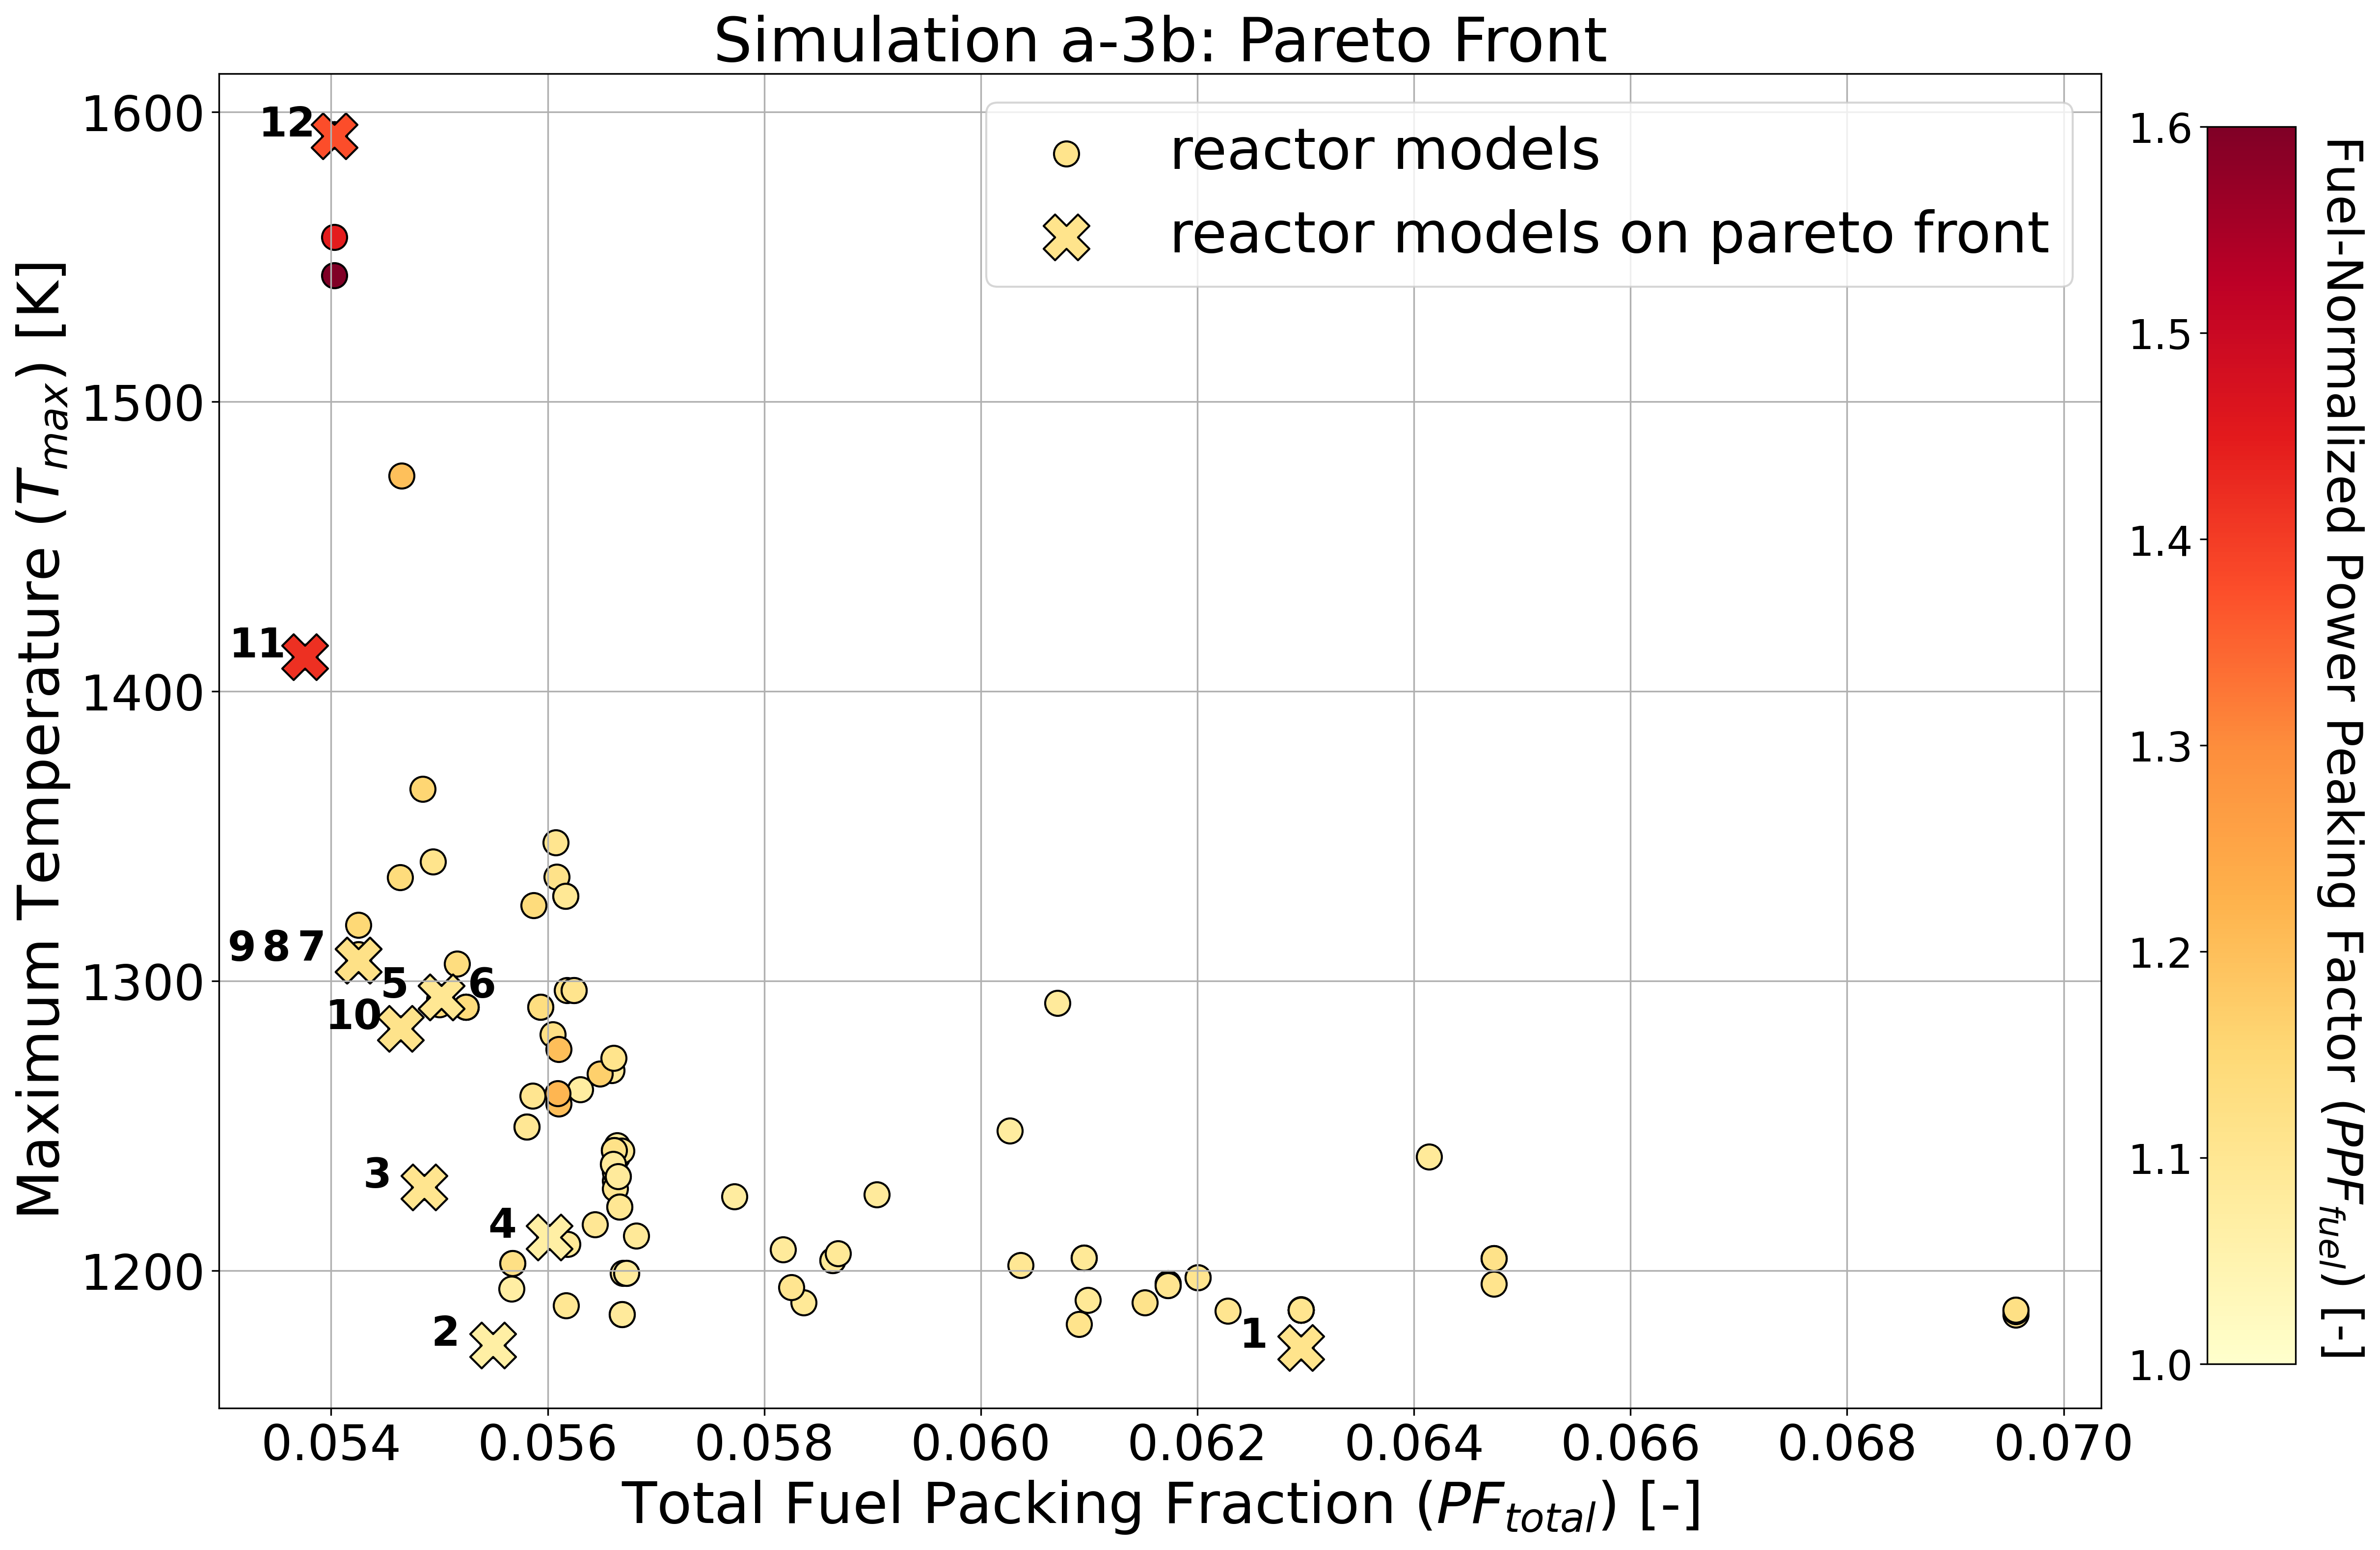
\includegraphics[width=\linewidth]{../docs/figures/assem-obj-3-all-2d.png} 
        \caption{Simulation a-3b: Plot of final generation's reactor models' 
        $PF_{total}$ against $T_{max}$ against $PPF_{fuel}$ as a color dimension. 
        Crosses indicate the reactor models on the Pareto front.}
    \end{figure}
    \end{column}
    \begin{column}{0.35\textwidth}
        \begin{block}{Simulation a-3b}
            \begin{itemize}
            \item Vary $PF_{total}$, \textbf{a, b, c, d, e f} ($\rho_{TRISO}(\vec{x}, 
            \vec{y}$)), and $r_1, r_2, r_3, r_4, r_5$ (coolant channel shape) 
            \item Minimize all three objectives: $PF_{total}$, $T_{max}$ and $PPF_{fuel}$.
            \item 6 generations 
            \item 128 reactor models per gen 
            \item Total runtime: 1528 Theta node-hours 
            \end{itemize}
            \end{block}
        \end{column}
\end{columns}
\end{frame}

\begin{frame}
    \frametitle{AHTR One-Third Assembly Simulation a-3b Results}
    \begin{columns}
        \begin{column}{0.7\textwidth}
    \begin{figure}
        \only<1>{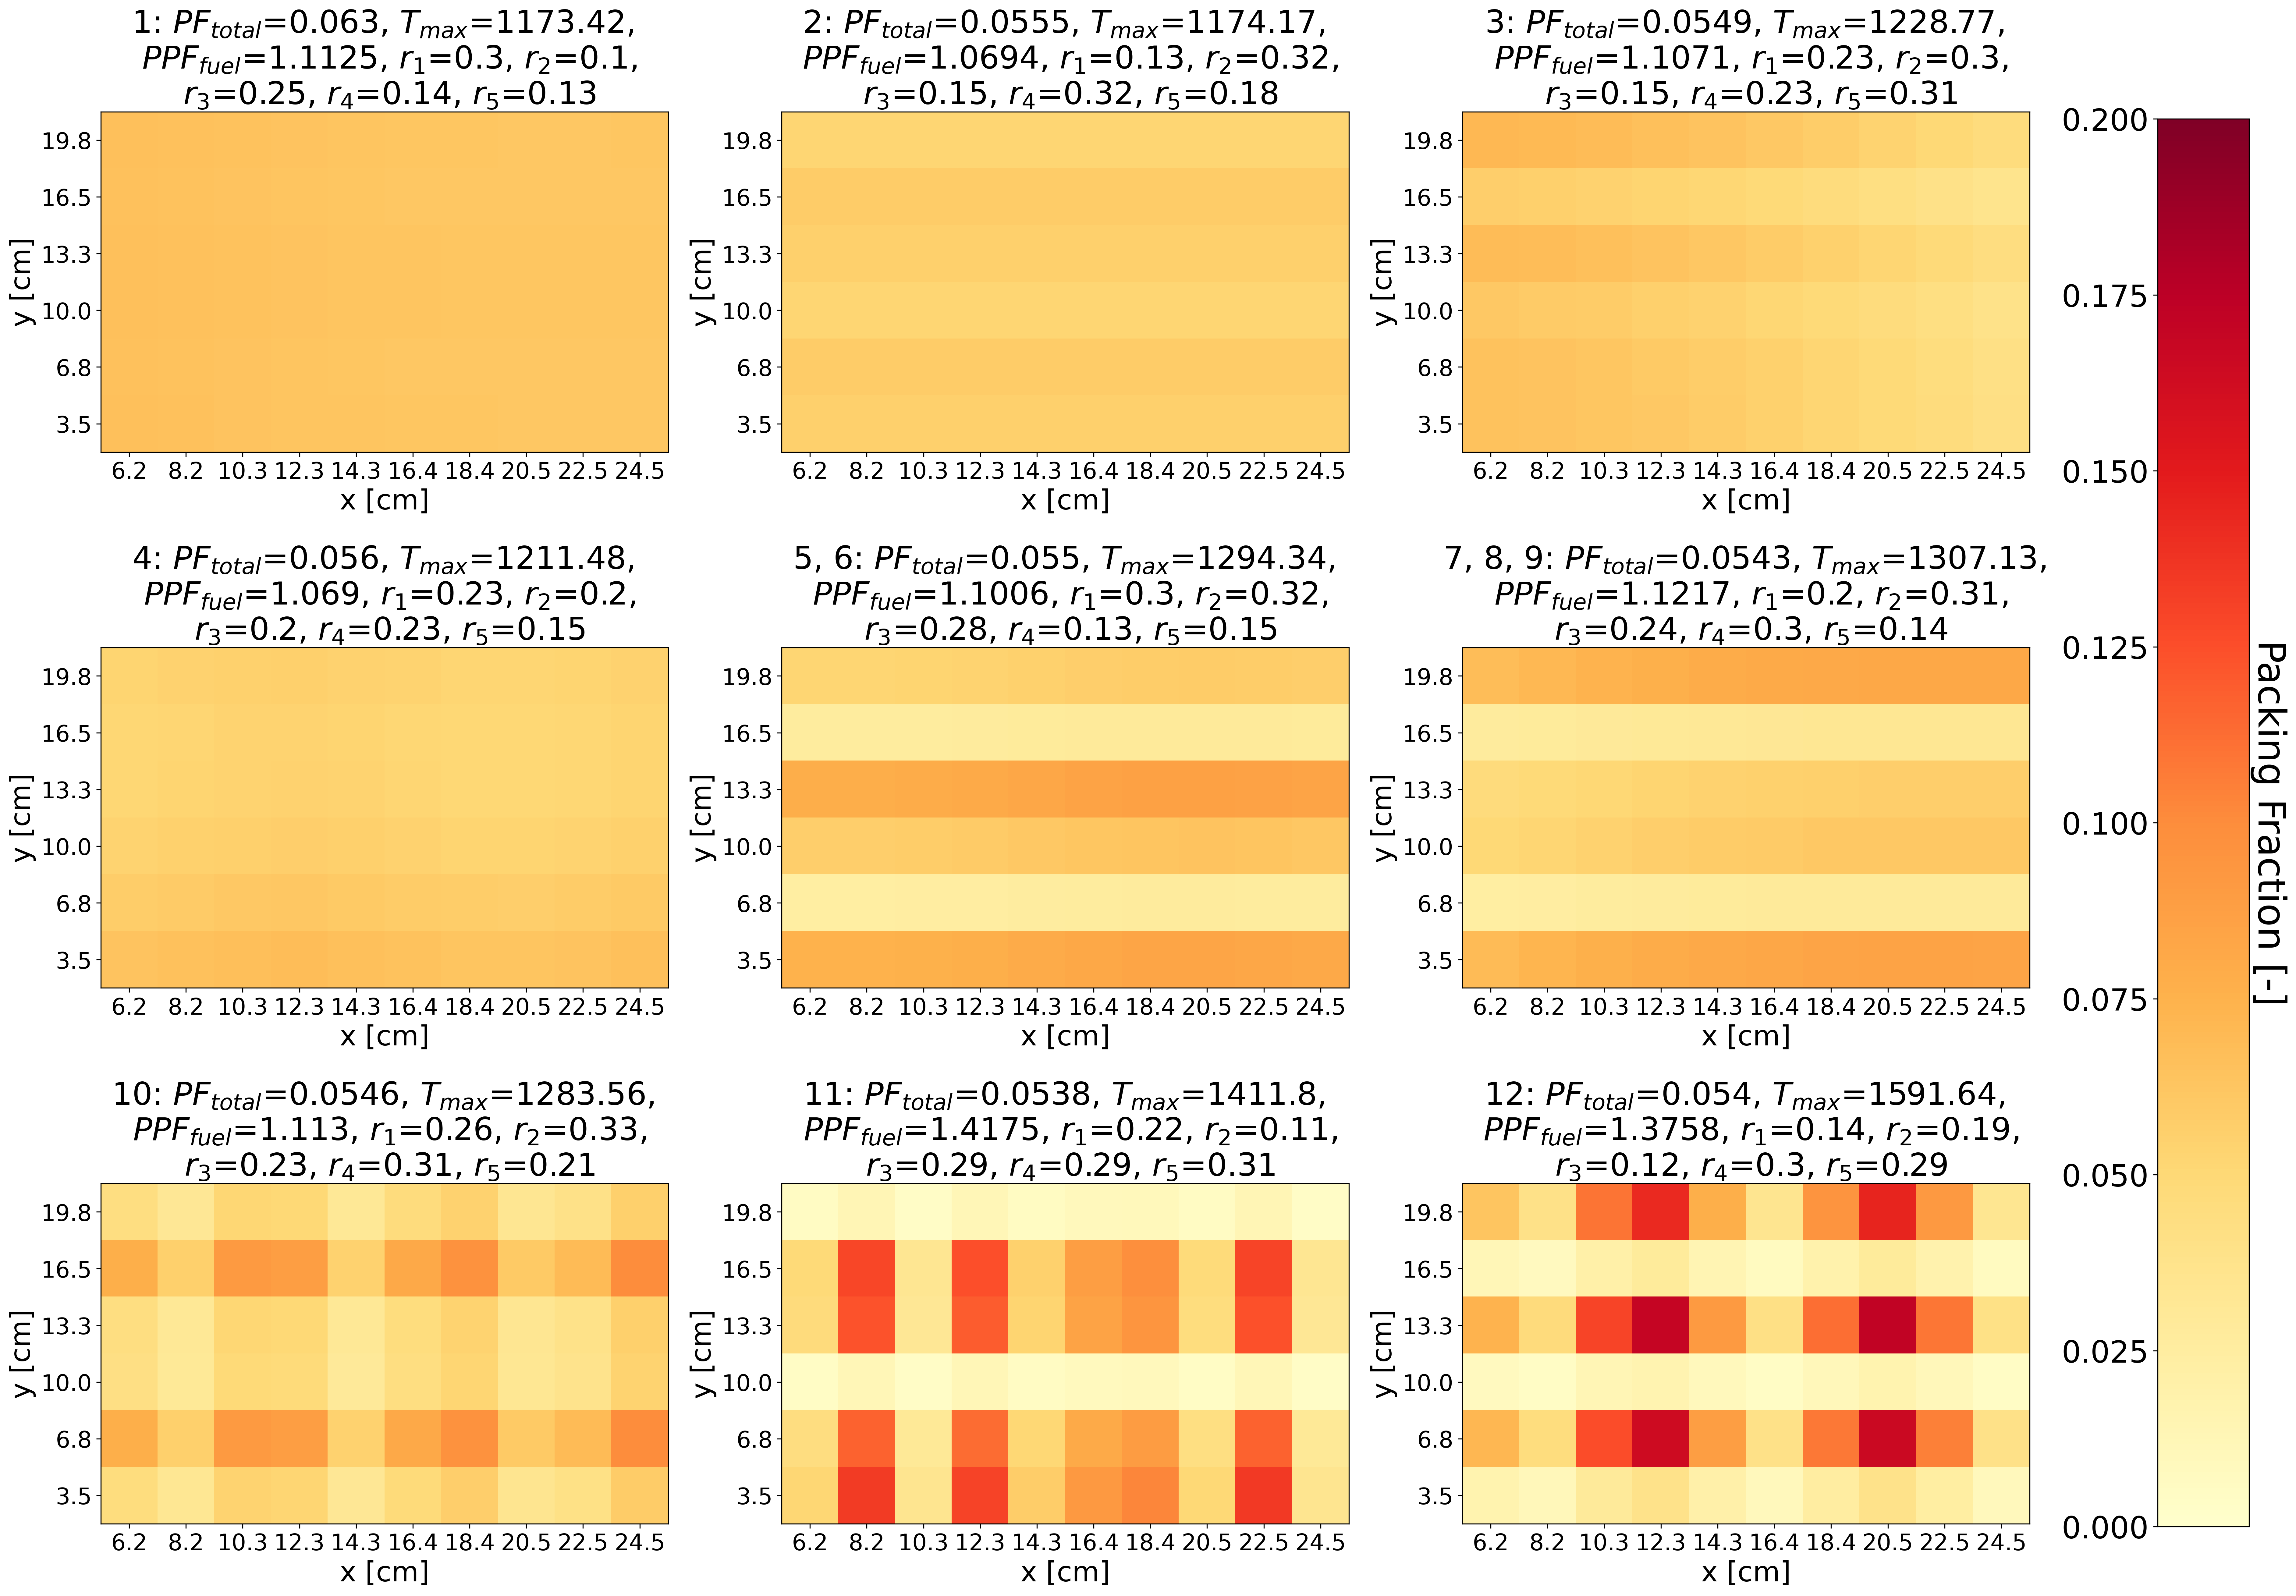
\includegraphics[width=0.8\linewidth]{../docs/figures/assem-obj-3-all-distr.png}}
        \only<2>{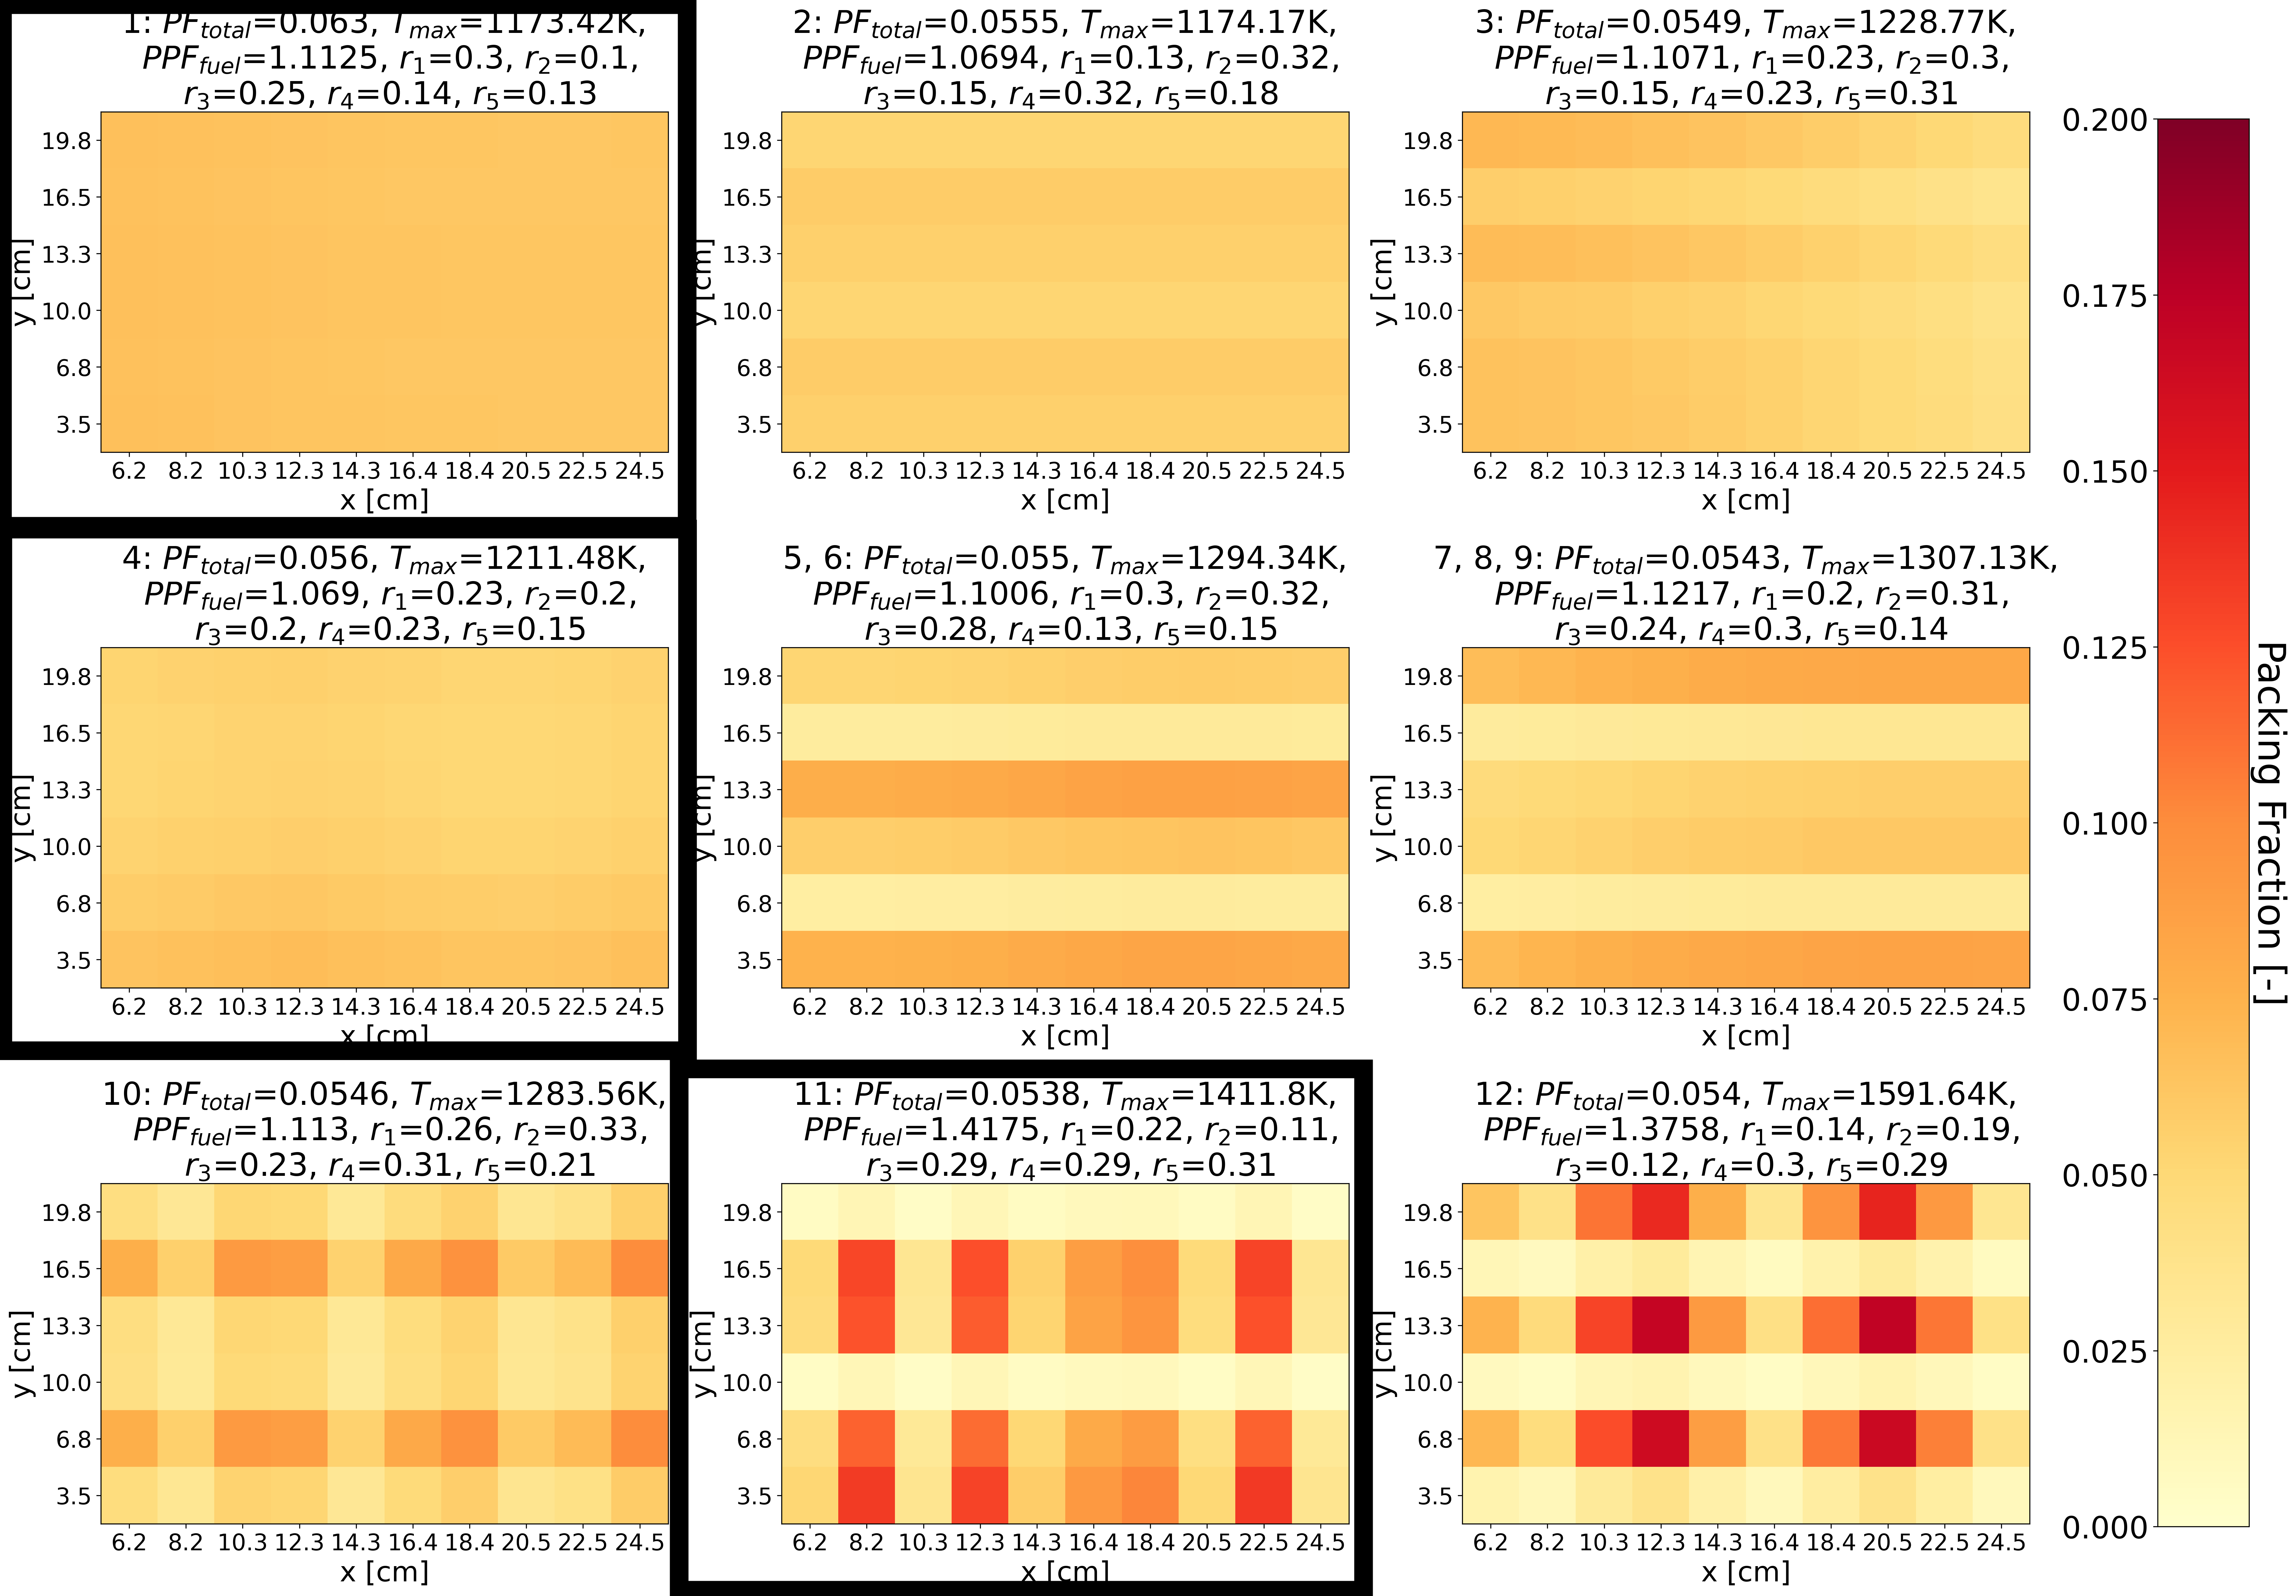
\includegraphics[width=0.8\linewidth]{figures/assem-obj-3-all-distr-annotated.png}}  
        \caption{TRISO distributions for the 12 reactor models on simulation 
        a-3b's Pareto front.}
    \end{figure}
\end{column}
\begin{column}{0.35\textwidth}
    \begin{block}{Simulation a-3b}
        \begin{itemize}
        \item Minimize $T_{max}$ objective: Flattens TRISO distribution and maximizes radius values 
        near temperature peaks 
        \item Minimize $PF_{total}$ and $PPF_{fuel}$ influence each other to have different 
        TRISO distributions at different $PF_{total}$ values 
        \end{itemize}
        \end{block}
    \end{column}
\end{columns}
\end{frame}

%\begin{frame}
%    \frametitle{AHTR One-Third Assembly Simulation a-3b Results}
%    \begin{figure}
%        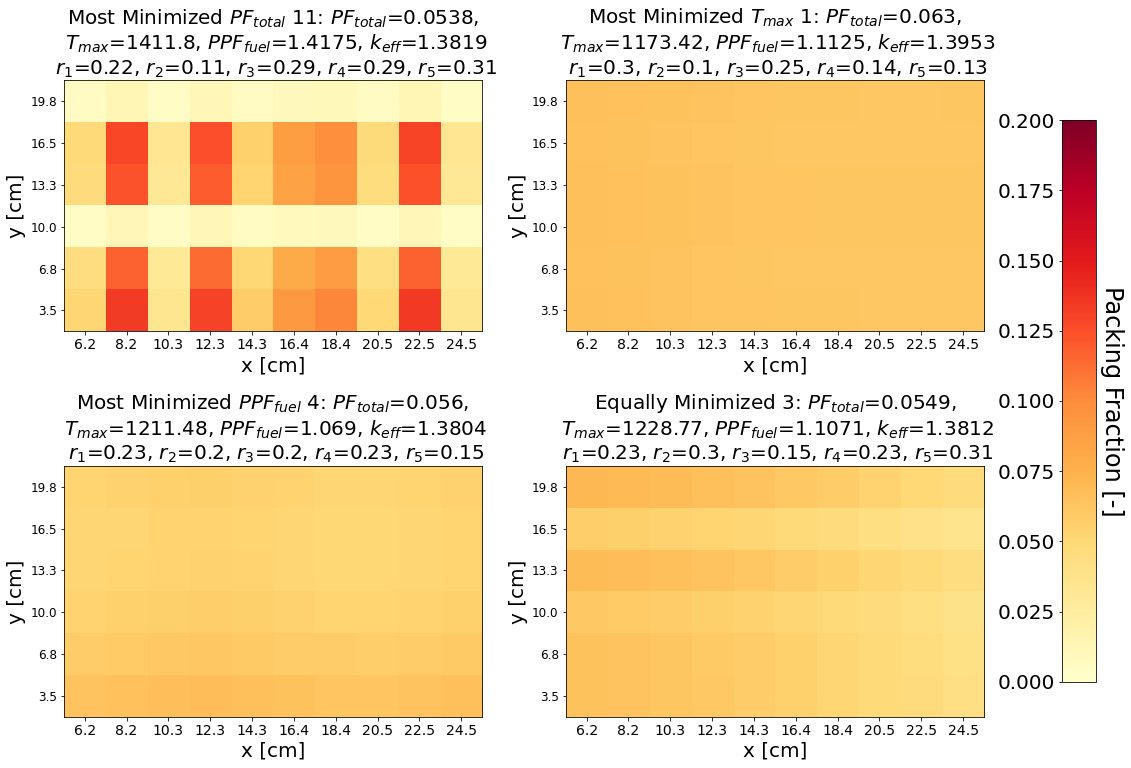
\includegraphics[width=0.8\linewidth]{../docs/figures/assem-obj-3-all-distr-most-minimized.png} 
%        \caption{Simulation a-3b: Plot of final generation's reactor models' 
%        $PF_{total}$ against $T_{max}$ against $PPF_{fuel}$ as a color dimension. 
%        Crosses indicate the reactor models on the Pareto front.}
%    \end{figure}
%\end{frame}

\begin{frame}
    \frametitle{AHTR One-Third Assembly Simulation a-3b Results}
    \begin{figure}
        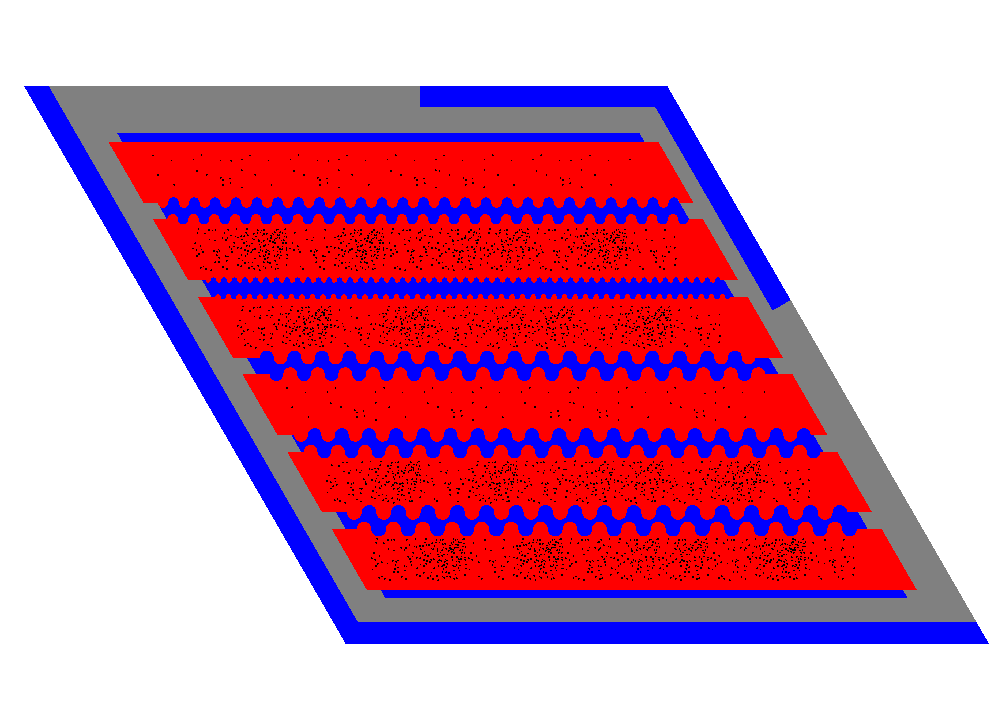
\includegraphics[width=0.7\linewidth]{../docs/figures/assem-obj-3-all-min-pf.png} 
        \caption{Simulation a-3b most minimized $PF_{total}$ reactor model's AHTR geometry.}
    \end{figure}
\end{frame}

\begin{frame}
    \frametitle{AHTR One-Third Assembly Optimization Simulations: Summary}
    \begin{block}{AHTR One-Third Assembly Optimization}
        \begin{itemize}
            \item The multi-objective optimization simulations successfully found a 
            wide spread of reactor models on their Pareto fronts that meet each 
            objective to varying degrees
            \item The $T_{max}$ objective flattens TRISO distribution and 
            maximizes radius values near temperature peaks 
            \item The $PF_{total}$ objective's driving factor maximize 
            total fission reaction rate and $PPF_{fuel}$ objective's driving 
            factor flattening thermal flux distribution influence each other resulting 
            in unexpected TRISO distributions at different $PF_{total}$ values 
        \end{itemize}
    \end{block}
    \begin{block}{ROLLO}
        \begin{itemize}
            \item  Results demonstrate ROLLO's success in conducting a multi-objective 
            global search of the large AHTR design space to find optimal reactor models 
            that satisfy all the objectives
        \end{itemize}
    \end{block}

\end{frame}